\documentclass[11pt,a4paper]{article}

\usepackage[utf8]{inputenc}
\usepackage[T5,T1]{fontenc}
\usepackage[vietnamese,english]{babel}
\usepackage[a4paper,top=20mm,bottom=20mm,left=25mm,right=20mm]{geometry}

\usepackage{amsmath,amssymb,amsfonts}
\usepackage{booktabs}
\usepackage{tabularx}
\usepackage{graphicx}
\usepackage{caption,subcaption}
\usepackage{enumitem}
\usepackage{xcolor}
\usepackage{titlesec}
\usepackage{algorithm}
\usepackage{algpseudocode}
\usepackage{setspace}

\usepackage[
    colorlinks=true,
    linkcolor=blue,
    citecolor=blue,
    urlcolor=blue
]{hyperref}

\onehalfspacing
\setlength{\parindent}{0pt}
\setlength{\parskip}{1.2ex}

\titlespacing*{\section}{0pt}{12pt}{6pt}
\titlespacing*{\subsection}{0pt}{10pt}{4pt}

\titleformat{\section}{\large\bfseries}{\thesection.}{0.5em}{}
\titleformat{\subsection}{\normalsize\bfseries}{\thesubsection.}{0.5em}{}

\begin{document}
\selectlanguage{vietnamese}

\begin{center}
    {\Large\bfseries BÁO CÁO TIẾN ĐỘ THỰC HIỆN KHÓA LUẬN TỐT NGHIỆP}
\end{center}

\vspace{0.4cm}

% ==============================================================================
% 1. NỘI DUNG ĐỀ TÀI
% ==============================================================================
\section{Nội dung đề tài}

Đề tài tập trung nghiên cứu, thiết kế và hiện thực hóa hệ thống dự đoán lưu lượng và điều khiển lưu lượng chủ động (Traffic Engineering) trong mạng diện rộng dựa trên sự kết hợp giữa học liên kết (Federated Learning) và học tăng cường sâu (Deep Reinforcement Learning).

Mô hình học máy dự báo mức sử dụng liên kết từ dữ liệu phân tán tại các miền mạng thông qua thuật toán tổng hợp FedAdam mà không cần chia sẻ dữ liệu gốc, bảo đảm tính riêng tư. Tác tử RecurrentPPO kết hợp kết quả dự đoán với trạng thái mạng hiện tại để ra quyết định chọn đường tối ưu trên tập K-Shortest Paths cho các luồng lưu lượng lớn, kết hợp cơ chế rơ-le trễ Schmitt-Trigger chống rung giật tuyến và cơ chế tự động chuyển hướng tức thời khi có sự cố đứt liên kết nhằm tối ưu hóa hiệu quả sử dụng tài nguyên và nâng cao chất lượng dịch vụ.

% ==============================================================================
% 2. CÁC NỘI DUNG ĐÃ THỰC HIỆN
% ==============================================================================
\section{Các nội dung đã thực hiện}

\subsection{Xây dựng mô hình mô phỏng mạng}
Đã chuẩn hóa và cấu hình mô hình mạng trên cả ba topo thực tế: NSFNET (14 router, 42 liên kết có hướng, băng thông 1 Gbps, trễ 2–10 ms), GÉANT (22 router, 72 liên kết có hướng, băng thông 2.5 Gbps), và Abilene (12 router, 30 liên kết có hướng, băng thông 1 Gbps). Mỗi topo được phân chia thành ba miền mạng độc lập (Domain A, B, C); mỗi miền đóng vai trò một FL Client huấn luyện mô hình dự báo từ dữ liệu cục bộ.

Môi trường huấn luyện Gymnasium (\texttt{rl/env.py}) đã được xây dựng hoàn chỉnh, tích hợp mô hình hàng đợi viễn thông M/M/1 để tính toán chính xác độ trễ lan truyền vật lý, độ trễ xếp hàng dựa trên mức độ chiếm dụng băng thông và xác định tỷ lệ mất gói tức thời khi hàng đợi vượt ngưỡng dung lượng.

\subsection{Xây dựng dữ liệu lưu lượng mạng}
Đã xây dựng chương trình sinh dữ liệu lưu lượng theo Mô hình Hấp dẫn (Gravity Model), mô phỏng chu kỳ ngày/đêm, suy giảm ngày cuối tuần, bùng phát tải cục bộ và sự cố đứt liên kết ngẫu nhiên qua chu kỳ 4 tuần với bước nhảy 15 phút.

Dữ liệu được tiền xử lý và cắt lát theo cửa sổ trượt gồm 12 bước quá khứ ($T=12$, tương đương 3 giờ) để dự đoán 3 bước trong tương lai ($H=3$, tương đương 45 phút nhìn trước) và phân chia theo 3 miền mạng phục vụ huấn luyện FL. Đồng thời, chuỗi ma trận lưu lượng thực nghiệm của GÉANT và Abilene đã được chuẩn hóa để kiểm thử khả năng thích ứng và chuyển giao mô hình.

\subsection{Xây dựng và thiết lập mô hình Federated Learning (TrafficLSTM)}
Đã triển khai kiến trúc học liên kết (Federated Learning) nhằm dự báo chủ động mức độ chiếm dụng của các liên kết mạng diện rộng (WAN) mà không xâm phạm quyền riêng tư dữ liệu lưu lượng giữa các miền tự trị (Autonomous Systems). Mỗi miền mạng hoạt động như một FL Client độc lập, huấn luyện mô hình dự báo cục bộ trên tập chuỗi thời gian của riêng mình, sau đó chỉ truyền tải sai phân trọng số mô hình về máy chủ trung tâm để tổng hợp thành mô hình toàn cục.

Về cấu trúc mạng và thiết lập mô hình \texttt{TrafficLSTM}:
\begin{itemize}[leftmargin=1.5em, itemsep=0.3ex]
    \item \textbf{Cửa sổ thời gian (Lookback \& Horizon):} Mô hình tiếp nhận chuỗi tải liên kết trong cửa sổ trượt quá khứ gồm 12 bước thời gian ($T = 12$, tương đương 3 giờ lịch sử với chu kỳ lấy mẫu 15 phút), và xuất ra dự báo mức tải tương lai cho 3 bước thời gian kế tiếp ($H = 3$, tương đương 45 phút nhìn trước).
    \item \textbf{Kiến trúc tầng ẩn và kỹ thuật điều hòa:} Sử dụng 2 tầng hồi quy LSTM với kích thước tầng ẩn 64 đơn vị (\texttt{hidden\_size} = 64), tích hợp lớp \texttt{Dropout} với tỷ lệ $p = 0.2$ giữa các tầng nhằm triệt tiêu hiện tượng quá khớp (overfitting) và tăng cường độ vững cáp (robustness) trước các xung đột biến tải. Trạng thái ẩn tại bước thời gian cuối cùng được đưa qua một tầng tuyến tính (Linear Projection Head) để suy luận tải dự phóng tương lai.
    \item \textbf{Đệm đặc trưng động (Dynamic Feature Padding):} Áp dụng kỹ thuật chèn số 0 để chuẩn hóa kích thước đầu vào của các miền mạng có số lượng liên kết khác nhau về cùng một chuẩn thống nhất mà không làm biến dạng phân phối dữ liệu gốc.
    \item \textbf{Tổng hợp thích nghi FedAdam trên FL Server:} Nhằm khắc phục hiện tượng trôi dạt trọng số (client drift) do dữ liệu lưu lượng giữa các miền mang bản chất dị thể phi đồng nhất (Non-IID), máy chủ trung tâm áp dụng thuật toán tối ưu hóa \texttt{FedAdam} với các hệ số động lượng thích nghi $\beta_1 = 0.9$ và $\beta_2 = 0.99$, giúp mô hình hội tụ ổn định và đạt sai số dự báo trung bình $\text{MAE} < 0.05$.
\end{itemize}

\begin{table}[htbp]
\centering
\caption{\textit{Bảng siêu tham số cấu hình mô hình Federated TrafficLSTM và thuật toán tổng hợp FedAdam.}}
\label{tab:fl_hyperparameters}
\small
\renewcommand{\arraystretch}{1.18}
\begin{tabularx}{\textwidth}{@{} p{4.2cm} c c X @{}}
\toprule
\textbf{Tham số cấu hình} & \textbf{Ký hiệu} & \textbf{Giá trị} & \textbf{Mô tả kỹ thuật \& Ý nghĩa} \\
\midrule
\multicolumn{4}{@{}l}{\textbf{1. Cửa sổ thời gian \& Kiến trúc mạng (TrafficLSTM)}} \\
Cửa sổ lịch sử trượt & $T$ & 12 bước & Chuỗi quan sát 3 giờ quá khứ ($12 \times 15\text{ phút}$). \\
Tầm nhìn dự báo tương lai & $H$ & 3 bước & Khoảng nhìn trước 45 phút ($3 \times 15\text{ phút}$) cho RL. \\
Số tầng hồi quy LSTM & $L$ & 2 tầng & Học phụ thuộc thời gian và tính tuần hoàn tải mạng. \\
Kích thước tầng ẩn & $d_{\text{hidden}}$ & 64 units & Dung lượng biểu diễn tối ưu, triệt tiêu nguy cơ quá khớp. \\
Tỷ lệ ngắt Dropout & $p_{\text{drop}}$ & 0.2 & Điều hòa kết nối giữa 2 tầng LSTM chống overfit. \\
Tầng xuất dữ liệu & FC & Tuyến tính & Chiếu trạng thái ẩn: $64 \to (H \times F_{\text{in}})$. \\
Đệm đặc trưng động & -- & Zero-Padding & Chuẩn hóa kích thước liên kết giữa các miền dị thể. \\
\midrule
\multicolumn{4}{@{}l}{\textbf{2. Huấn luyện Client \& Tối ưu hóa FedAdam}} \\
Kích thước mini-batch & $B_{\text{FL}}$ & 32 mẫu & Kích thước lô huấn luyện cục bộ tại mỗi miền mạng. \\
Epoch cục bộ mỗi vòng & $E$ & 5 epochs & Cân bằng giữa tính toán biên và băng thông truyền thông. \\
Tốc độ học cục bộ & $\eta_{\text{local}}$ & $1 \times 10^{-3}$ & Bộ tối ưu Adam, hàm mất mát sai số bình phương (MSE). \\
Tốc độ học máy chủ & $\eta_{\text{global}}$ & $1 \times 10^{-3}$ & Cập nhật mô hình toàn cục trên máy chủ điều phối. \\
Động lượng FedAdam & $\beta_1, \beta_2$ & 0.9, 0.99 & Bù đắp trôi dạt trọng số do dữ liệu phân tán Non-IID. \\
Tham số ổn định số học & $\tau$ & $1 \times 10^{-3}$ & Tránh hiện tượng chia cho 0 trong bộ tiền điều kiện. \\
Vòng giao tiếp toàn cục & $R$ & 50 vòng & Đạt trạng thái hội tụ với sai số dự báo $\text{MAE} < 0.05$. \\
\bottomrule
\end{tabularx}
\end{table}

\subsection{Xây dựng và thiết lập môi trường Reinforcement Learning (RecurrentPPO)}
Đã hoàn thiện môi trường Gymnasium (\texttt{rl/env.py}) để phục vụ huấn luyện tác tử điều khiển lưu lượng theo cơ chế tối ưu hóa vòng lặp kín (Closed-Loop Autonomous Routing). Thiết lập kỹ thuật của môi trường và tác tử bao gồm các điểm then chốt:

\begin{itemize}[leftmargin=1.5em, itemsep=0.3ex]
    \item \textbf{Không gian trạng thái (Observation Space) và Cơ chế nạp dự báo (State Space Injection):} Không gian quan sát của tác tử được cấu thành thông qua phép ghép nối đặc trưng (Feature Concatenation) giữa ba thành phần thông tin trọng yếu:
    \begin{equation}
        \mathbf{s}_t = \left[ \mathbf{u}_t \;\parallel\; \mathbf{\hat{u}}_{t+1} \;\parallel\; \mathbf{d}_t \right]
    \end{equation}
    trong đó $\mathbf{u}_t$ là mức tải thực tế hiện tại của các liên kết, $\mathbf{d}_t$ là nhu cầu lưu lượng tức thời của các luồng lớn, và đặc biệt $\mathbf{\hat{u}}_{t+1}$ là \textbf{vector tải dự phóng ở bước kế tiếp do mô hình Federated TrafficLSTM cung cấp}. Cơ chế nạp dự báo này trang bị cho tác tử năng lực phán đoán chủ động, cho phép điều chuyển luồng giải tỏa nguy cơ tắc nghẽn từ trước khi hàng đợi gói tin bị phình to.
    
    \item \textbf{Không gian hành động đa rời rạc (Multi-Discrete Action Space) theo nguyên lý Pareto 80/20:} Thay vì điều khiển toàn bộ ma trận lưu lượng (gây bùng nổ tổ hợp không gian hành động), hệ thống áp dụng nguyên lý 80/20 chỉ tập trung kiểm soát nhóm luồng lưu lượng trọng yếu (Elephant Flows / Heavy-Hitters chiếm trên 85\% tổng tải): 20 luồng trên NSFNET, 30 luồng trên GÉANT và 15 luồng trên Abilene. Với mỗi luồng này, thuật toán Yen tiền tính toán $K = 3$ đường đi ngắn nhất không lặp vòng (\texttt{K-Shortest Paths}). Tác tử lựa chọn hành động trong không gian \texttt{MultiDiscrete([3, ..., 3])}, trong khi các luồng nhỏ còn lại mặc định phân bổ trên tuyến ngắn nhất OSPF.

    \item \textbf{Kiến trúc mạng chính sách RecurrentPPO (MlpLstmPolicy):} Tác tử sử dụng kiến trúc Actor-Critic kết hợp tầng nhớ LSTM kích thước 128 đơn vị. Khác với thuật toán PPO phản xạ không trạng thái (dễ đưa ra quyết định đổi tuyến liên tục khi tải dao động nhẹ quanh ngưỡng), tầng nhớ LSTM lưu giữ vết ngữ cảnh định tuyến và thiết lập nên \textbf{quán tính hành động (Action Inertia)}, giúp triệt tiêu hoàn toàn hiện tượng rung giật tuyến (Route Flapping), giữ tỷ lệ nhảy tuyến (Route Churn) ở mức ổn định dưới 0.1\% mà vẫn bảo đảm phản xạ tức thời khi có sự cố đứt liên kết.
\end{itemize}

\begin{figure}[htbp]
    \centering
    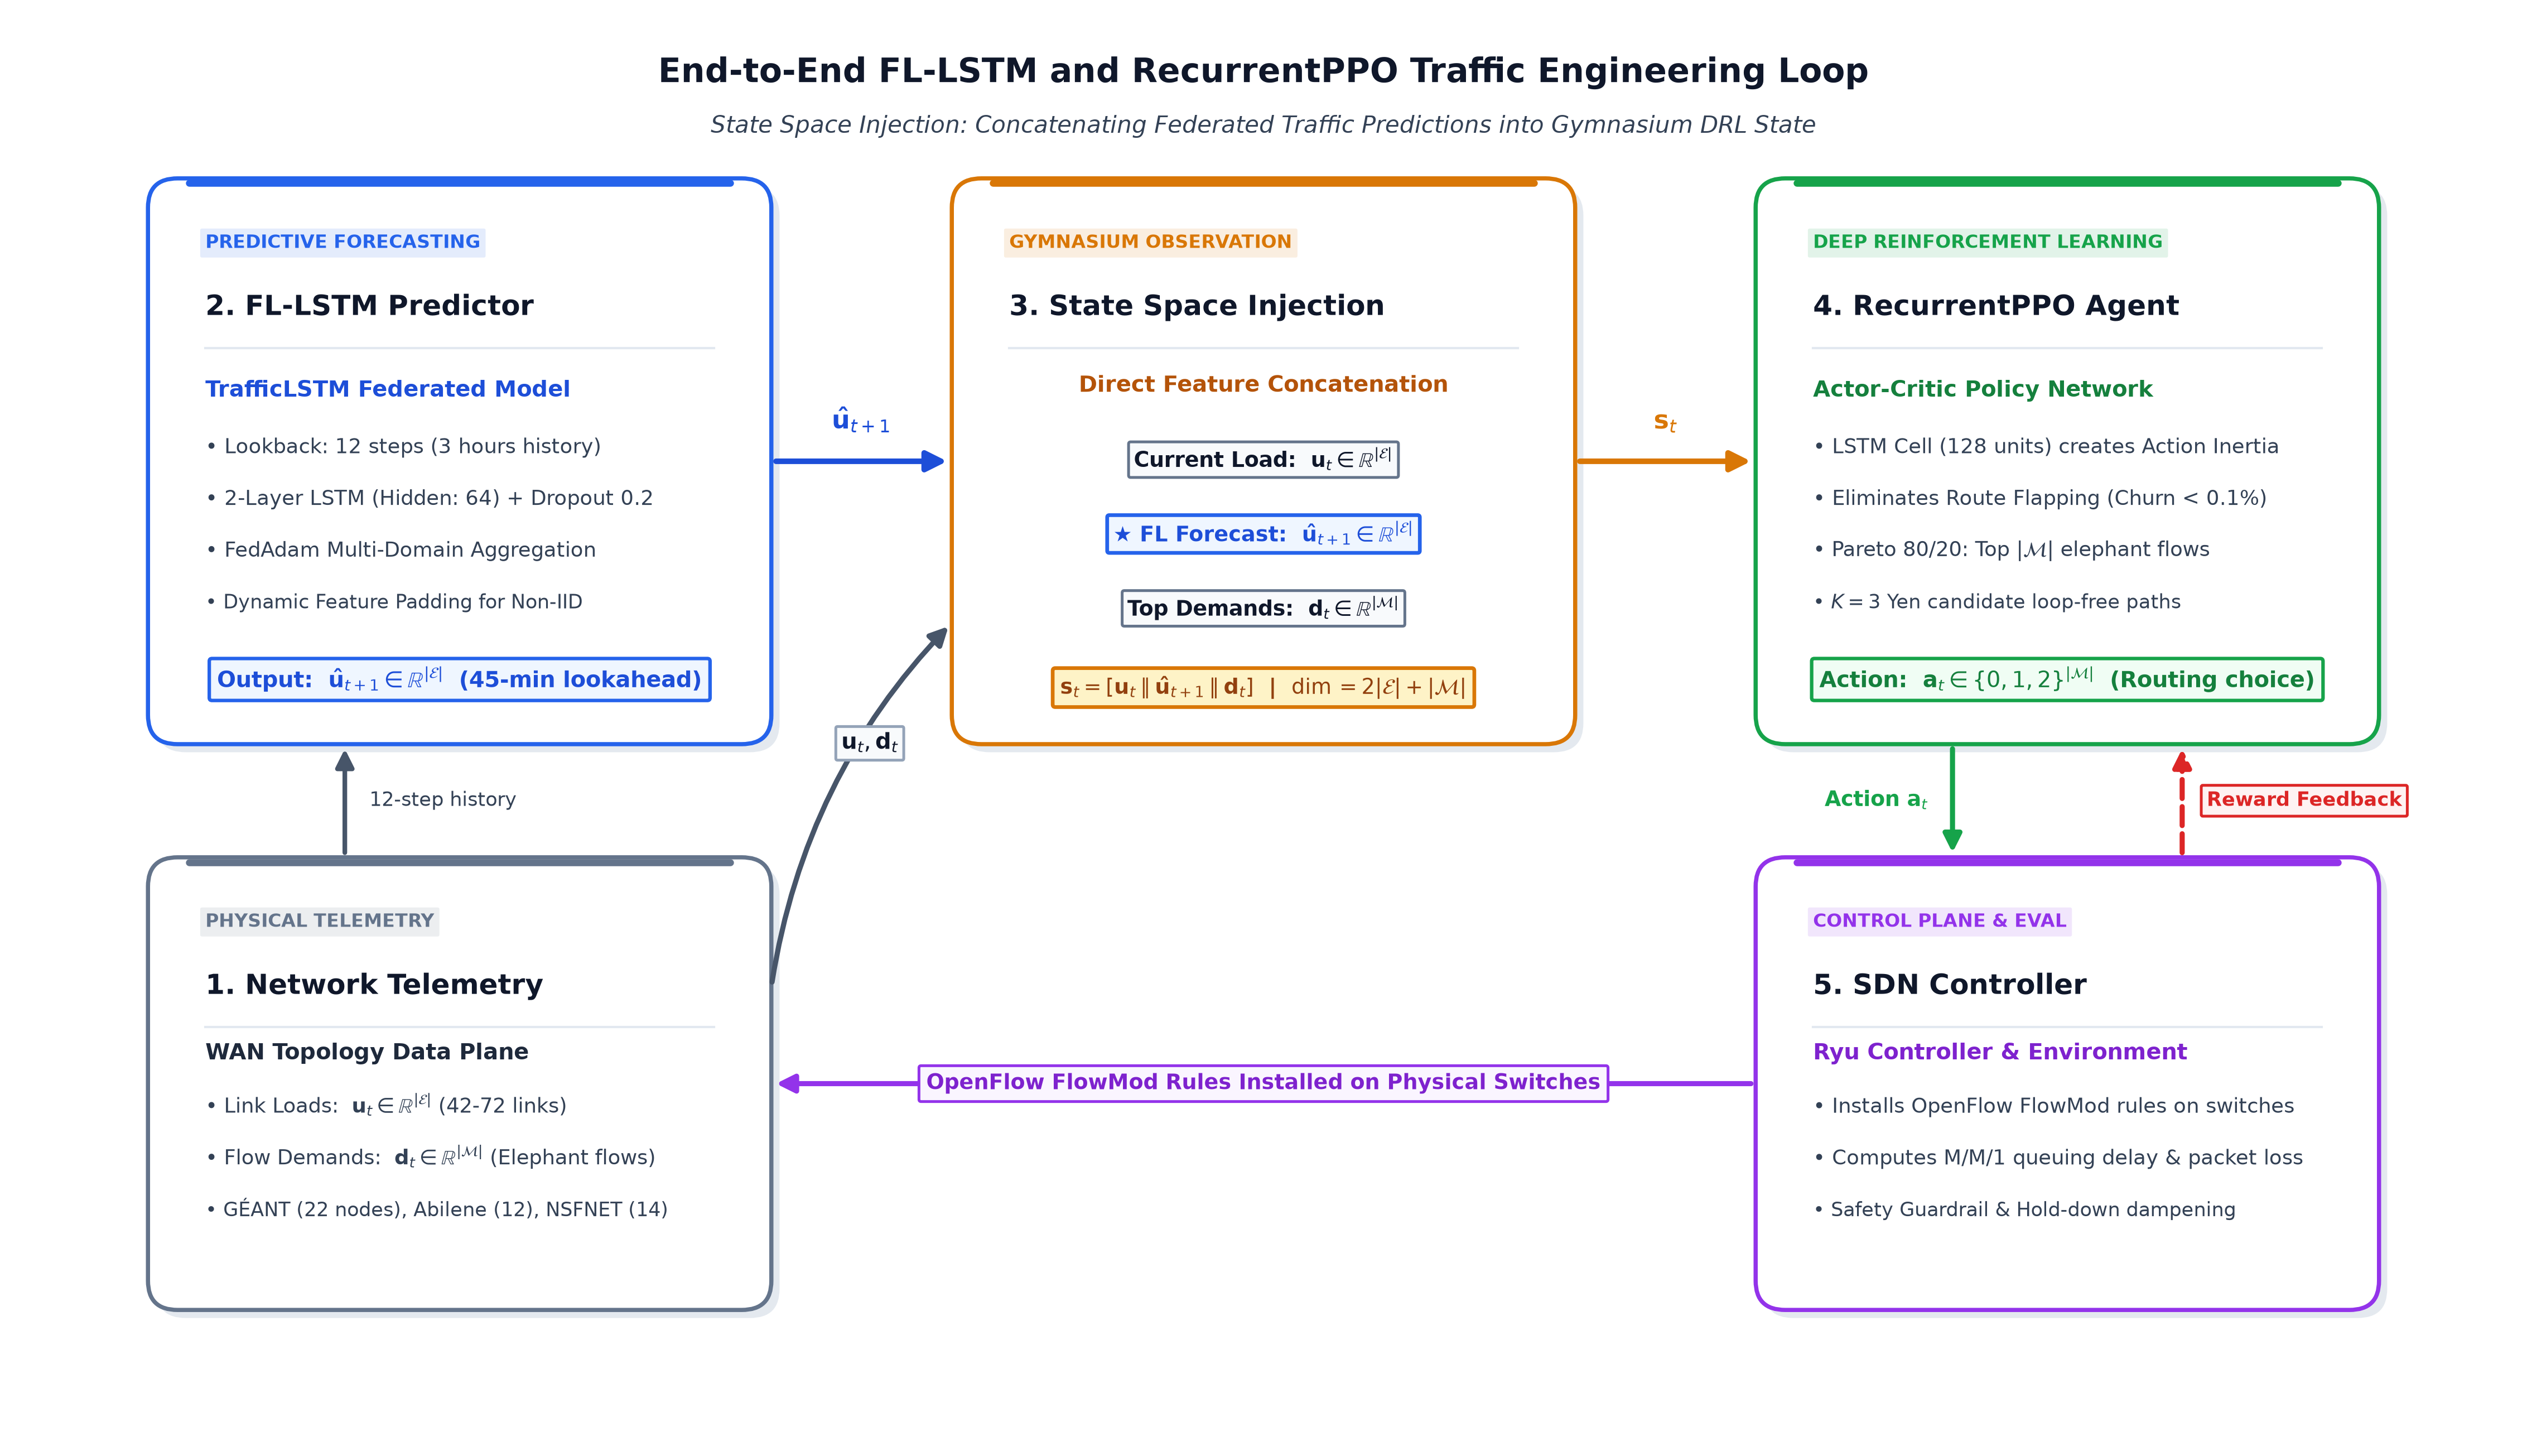
\includegraphics[width=0.96\textwidth]{figures/fig_lstm_ppo_env.png}
    \caption{\textit{Sơ đồ tích hợp hệ thống điều khiển lưu lượng chủ động: Dữ liệu tải quá khứ được mô hình Federated TrafficLSTM dự báo và nạp vào không gian trạng thái của môi trường Gymnasium (State Space Injection), cung cấp đầu vào cho tác tử RecurrentPPO đưa ra quyết định định tuyến tối ưu khép kín thông qua bộ điều khiển SDN.}}
    \label{fig:lstm_ppo_env}
\end{figure}

\begin{table}[htbp]
\centering
\caption{\textit{Bảng siêu tham số cấu hình tác tử điều khiển định tuyến \texttt{RecurrentPPO} và hàm phần thưởng.}}
\label{tab:rl_hyperparameters}
\small
\renewcommand{\arraystretch}{1.18}
\begin{tabularx}{\textwidth}{@{} p{4.2cm} c c X @{}}
\toprule
\textbf{Tham số cấu hình} & \textbf{Ký hiệu} & \textbf{Giá trị} & \textbf{Mô tả kỹ thuật \& Ý nghĩa} \\
\midrule
\multicolumn{4}{@{}l}{\textbf{1. Kiến trúc mạng chính sách (Policy Network - MlpLstmPolicy)}} \\
Lớp chính sách & -- & \texttt{MlpLstm} & Actor-Critic tích hợp tầng nhớ trạng thái ẩn LSTM. \\
Tầng nhớ trạng thái ẩn & $d_{\text{lstm}}$ & 128 units & Tạo quán tính hành động (Action Inertia) chống rung giật. \\
Mạng Actor ($\pi_\theta$) & MLP & $[256, 128]$ & Đầu ra phân phối xác suất Softmax chọn tuyến Yen $K=3$. \\
Mạng Critic ($V_\phi$) & MLP & $[256, 128]$ & Đầu ra vô hướng ước lượng hàm giá trị trạng thái $V(\mathbf{s}_t)$. \\
\midrule
\multicolumn{4}{@{}l}{\textbf{2. Quá trình tối ưu hóa RecurrentPPO \& GAE}} \\
Bộ đệm Rollout & $N_{\text{steps}}$ & 1024 bước & Thu thập 128 bước trên 8 môi trường mạng song song. \\
Kích thước mini-batch & $B_{\text{RL}}$ & 64 mẫu & Kích thước lô chuyển trạng thái trong mỗi pha tối ưu. \\
Epoch cập nhật & $K_{\text{epoch}}$ & 10 epochs & Số lượt huấn luyện lặp lại trên bộ đệm rollout. \\
Lập lịch tốc độ học & $\alpha$ & $3 \cdot 10^{-4} \to 1 \cdot 10^{-4}$ & Suy giảm tuyến tính theo tiến trình học tổng thể. \\
Hệ số chiết khấu & $\gamma$ & 0.95 & Cân bằng giữa tối ưu tức thời và rủi ro nghẽn dài hạn. \\
Hệ số lợi thế GAE & $\lambda_{\text{GAE}}$ & 0.95 & Kiểm soát phương sai và độ lệch của hàm ước lượng lợi thế. \\
Ngưỡng cắt tỉa PPO & $\epsilon_{\text{clip}}$ & 0.2 & Giới hạn biên độ thay đổi chính sách trong vùng tin cậy. \\
Hệ số mất mát Critic & $c_1$ & 0.5 & Trọng số tổn thất hàm giá trị trong tổng hàm mất mát. \\
Hệ số Entropy & $c_2$ & 0.001 & Kiểm soát thăm dò, ưu tiên khai thác chính sách tối ưu. \\
Cắt tỉa Gradient & $g_{\text{max}}$ & 0.5 & Giới hạn chuẩn gradient chống bùng nổ gradient trong LSTM. \\
\midrule
\multicolumn{4}{@{}l}{\textbf{3. Không gian hành động \& Hàm phần thưởng môi trường}} \\
Luồng kiểm soát trọng yếu & $|\mathcal{M}|$ & 20 / 30 / 15 & Quy tắc Pareto 80/20 trên NSFNET / GÉANT / Abilene. \\
Số tuyến ứng viên Yen & $K$ & 3 tuyến & Tập đường đi ngắn nhất không lặp vòng ($p_0, p_1, p_2$). \\
Trọng số phạt tải đỉnh & $w_{\text{MLU}}$ & 1.0 & Phạt tuyến tính ép tải cực đại dưới ngưỡng nghẽn. \\
Trọng số phạt trễ gói & $w_{\text{delay}}$ & 0.5 & Tối thiểu hóa độ trễ lan truyền và độ trễ xếp hàng. \\
Trọng số phạt mất gói & $w_{\text{loss}}$ & 40.0 & Ưu tiên hàng đầu: bảo vệ gói tin khi tiệm cận tắc nghẽn. \\
Trọng số phạt nhảy tuyến & $w_{\text{churn}}$ & 0.08 & Triệt tiêu hoàn toàn hiện tượng rung giật đường truyền. \\
Phạt trễ thích nghi & $w_{\text{excess}}$ & 0.8 / 0.3 & Chặt chẽ khi tải an toàn, nới lỏng khi tiệm cận ngưỡng nghẽn. \\
Bộ đệm giữ tuyến an toàn & $T_{\text{hold}}$ & $\ge 15$ bước & Khóa tuyến tối thiểu chống dao động tuyến ping-pong. \\
\bottomrule
\end{tabularx}
\end{table}

\subsection{Xây dựng hàm đánh giá môi trường}
Đã xây dựng và chuẩn hóa toàn bộ logic của hàm \texttt{step()} để mô phỏng trạng thái mạng sau mỗi quyết định định tuyến: ánh xạ hành động sang bảng tuyến, cộng dồn lưu lượng lên từng liên kết, tính mức sử dụng liên kết cực đại (MLU), tính toán độ trễ lan truyền, độ trễ hàng đợi và tỷ lệ mất gói theo mô hình M/M/1, đồng thời cập nhật tỷ lệ nhảy tuyến (Route Churn) và tính phần thưởng.

Quy trình thực thi logic chuyển trạng thái của môi trường Gymnasium được chuẩn hóa tường minh tại Thuật toán \ref{alg:gym_step}:

\begin{algorithm}[htbp]
\caption{Gymnasium Routing Environment Step Logic}
\label{alg:gym_step}
\begin{algorithmic}[1]
\Require Action vector $\mathbf{a}_t$, current traffic demand matrix $\mathbf{TM}_t$.
\Ensure Next state $\mathbf{s}_{t+1}$, reward $R_t$, termination flag $done$, diagnostics $info$.
\Statex \textbf{Phase 1: Flow Path Assignment}
\State Assign chosen path $p = \mathbf{a}_t[k]$ from $K$-shortest paths for each managed flow $k$.
\State Assign default shortest path (Path 0) to all remaining unmanaged background flows.
\Statex \textbf{Phase 2: Link Load Aggregation \& Queuing Simulation}
\State Sum traffic demands over all traversed links: $Demand(e) \gets \sum_{(u, v): e \in P_{(u,v)}} \mathbf{TM}_t[u, v]$.
\State Compute link utilization: $u(e) \gets Demand(e) \,/\, Capacity(e)$, and peak utilization: $\text{MLU}_t \gets \max_{e} u(e)$.
\State Compute latency and packet loss on each link using the M/M/1 queuing model.
\Statex \textbf{Phase 3: Route Stability \& Reward Computation}
\State Measure route flapping (churn): ratio of managed flows switching paths from $\mathbf{a}_{t-1}$.
\State Adapt delay penalty: $w_{\text{delay}} \gets 0.8$ if $\text{MLU}_t < 0.65$ (idle network), else $0.3$ (congested).
\State Calculate scalar reward $R_t$ based on MLU, delay, packet loss, and churn (Eq.~\ref{eq:reward}).
\Statex \textbf{Phase 4: FL Prediction Injection \& Observation Packaging}
\State Query Federated TrafficLSTM to obtain predicted future link load vector $\mathbf{\hat{u}}_{t+1}$.
\State Assemble next observation: $\mathbf{s}_{t+1} \gets [\text{current load } \mathbf{u}_t, \; \text{predicted load } \mathbf{\hat{u}}_{t+1}, \; \text{flow demand } \mathbf{d}_t]$.
\State \Return $(\mathbf{s}_{t+1}, R_t, done, info)$
\end{algorithmic}
\end{algorithm}

Hàm phần thưởng (Reward) được thiết kế đa mục tiêu phụ thuộc trạng thái nhằm tối ưu đồng thời nhiều chỉ số chất lượng dịch vụ SLA:
\begin{equation}
\label{eq:reward}
    R_t = -\left( 1.0 \cdot \text{MLU}_t + 0.5 \cdot \bar{D}_t^{norm} + w_{delay}^{excess}(t) \cdot D_t^{excess} + 3.0 \cdot \bar{L}_t + 0.08 \cdot \text{Churn}_t \right)
\end{equation}

Lý giải khoa học và căn cứ định lượng lựa chọn các tham số trong hàm phần thưởng:
\begin{itemize}[leftmargin=1.5em, itemsep=0.3ex]
    \item \textbf{Trọng số phạt mất gói ($3.0 \cdot \bar{L}_t$):} Đặt ở mức 3.0 vì nếu chọn thấp hơn (như 1.0), tác tử sẽ xem nhẹ việc mất gói và sẵn sàng đánh đổi làm rớt gói để duy trì độ trễ thấp; ngược lại nếu chọn quá cao (như 10.0), các đỉnh mất gói đột biến sẽ tạo ra gradient quá lớn làm mất ổn định quá trình tối ưu và gây sụp đổ chính sách.
    \item \textbf{Ngưỡng quá tải liên kết ($\text{MLU} = 0.65$):} Thiết lập ngưỡng ở 0.65 vì nếu chọn thấp hơn (như 0.50), hệ thống sẽ chuyển luồng quá sớm ngay cả khi mạng còn rất nhiều băng thông nhàn rỗi; còn nếu chọn cao hơn (như 0.80), hàng đợi liên kết bước vào vùng tăng trưởng phi tuyến làm độ trễ tăng vọt trước khi tác tử kịp điều phối.
    \item \textbf{Trọng số phạt trễ thích nghi khi mạng nhàn rỗi ($w_{delay} = 0.8$ khi $\text{MLU} < 0.65$):} Đặt ở mức 0.8 nhằm phạt nặng hành vi đi đường phụ dài hơn để ép toàn bộ luồng chạy trên đường ngắn nhất OSPF; nếu chọn thấp hơn (như 0.4), tác tử sẽ tùy tiện rẽ luồng gây tăng trễ vô ích, còn nếu chọn cao hơn (như 1.5), tác tử trở nên quá cứng nhắc và chậm thích nghi khi lưu lượng bắt đầu dâng cao.
    \item \textbf{Trọng số phạt trễ thích nghi khi mạng có nguy cơ nghẽn ($w_{delay} = 0.3$ khi $\text{MLU} \ge 0.65$):} Giảm xuống 0.3 nhằm nới lỏng phạt trễ, bật đèn xanh cho tác tử rẽ luồng sang tuyến phụ để cứu gói tin; nếu chọn thấp hơn (như 0.1), tác tử sẽ chọn những tuyến phụ quá dài làm bùng nổ độ trễ toàn mạng, còn nếu chọn cao hơn (như 0.6), tác tử sẽ sợ bị phạt trễ mà không dám chuyển luồng, khiến nghẽn mạng trầm trọng hơn.
    \item \textbf{Trọng số phạt nhảy tuyến ($0.08 \cdot \text{Churn}_t$):} Đặt ở mức 0.08 để cân bằng độ ổn định định tuyến; nếu chọn thấp hơn (như 0.02), tác tử sẽ đổi tuyến liên tục giữa các bước thời gian gây xáo trộn thứ tự gói tin (packet reordering), còn nếu chọn cao hơn (như 0.30), tác tử sẽ rơi vào trạng thái trơ và từ chối đổi tuyến ngay cả khi liên kết chính đang bị nghẽn nặng.
    \item \textbf{Bộ điều khiển rơ-le trễ Schmitt-Trigger và cơ chế SDN Failover:} Ngưỡng trễ $\tau_{high} = 0.65$ ngăn ngừa hiện tượng dao động qua lại giữa hai tuyến khi tải bấp bênh quanh ngưỡng; đồng thời cơ chế failover tự động phát hiện đứt cáp và chuyển hướng tức thời các luồng bị ảnh hưởng sang tuyến thay thế ngắn nhất (Bypass Path 0), giữ vững tỷ lệ mất gói bằng 0.00\%.
\end{itemize}

\subsection{Xây dựng pipeline thực nghiệm và đặc tả các kịch bản đánh giá}
Đã xây dựng pipeline hoàn chỉnh gồm các pha khép kín: sinh dữ liệu ma trận lưu lượng $\to$ tiền xử lý $\to$ huấn luyện FL $\to$ điều phối DRL $\to$ đánh giá đa kịch bản. Các script thực thi chính gồm \texttt{run\_full\_pipeline.py} và \texttt{demo.py}; mô hình huấn luyện được lưu trữ tập trung tại thư mục \texttt{models/}.

Bộ 6 kịch bản thực nghiệm được chuẩn hóa trên chu kỳ đánh giá $N_{\text{steps}} = 100$ bước ($\Delta t = 15$ phút/bước, tương đương 25 giờ liên tục). Gọi $\mathbf{D}_t$ là ma trận nhu cầu lưu lượng tức thời và $\mathbf{D}_t^{\text{base}}$ là ma trận chu kỳ danh định:

\begin{itemize}[leftmargin=1.5em, itemsep=0.4ex]
    \item \textbf{T1 (Nominal Traffic):} $\mathbf{D}_t = \mathbf{D}_t^{\text{base}}$ ($t \in [0, 99]$) -- Mô phỏng chu kỳ tải ngày/đêm tự nhiên, kiểm tra trễ tối ưu khi mạng vận hành ở vùng tải an toàn ($\text{MLU} < 0.65$).
    \item \textbf{T2 (Traffic Spike):} $\mathbf{D}_t(u, v) = 3.0 \cdot \mathbf{D}_t^{\text{base}}(u, v)$ trên top-3 luồng voi tại khung cao điểm ($t \in [30, 40]$) -- Kiểm tra phản xạ né nghẽn sớm nhờ vector dự báo tải $\hat{\mathbf{u}}_{t+1}$.
    \item \textbf{T3 (Gradual Escalation):} $\mathbf{D}_t = (1.0 + 0.5 \cdot \frac{t}{100}) \mathbf{D}_t^{\text{base}}$ ($t \in [0, 99]$) -- Tăng tải lũy tiến toàn mạng từ $+0\%$ lên $+50\%$, ép các liên kết chạm ngưỡng bão hòa để khảo sát khả năng chống rớt gói.
    \item \textbf{T4 (Flash Crowd):} $\mathbf{D}_t(u, v) = 5.0 \cdot \mathbf{D}_t^{\text{base}}(u, v)$ trên top-5 luồng voi tại $t \in [50, 55]$ -- Thử thách năng lực hấp thụ sốc tải đột biến cực hạn.
    \item \textbf{T5 (Link Failure):} Đứt liên kết lõi $e_{\text{crit}}$ tại bước $t = 15..60$ ($e_{\text{crit}} = (4, 7)$ trên GÉANT; $(1, 2)$ trên NSFNET) -- Kiểm tra cơ chế SDN Failover chuyển tuyến tức thời bảo toàn luồng không gián đoạn.
    \item \textbf{T6 (Irregular Day):} Tải phân bố lệch pha bất đối xứng: sáng dồn tải nặng $2.0 \cdot \mathbf{D}_t^{\text{base}}$ ($t \le 40$), trưa chuẩn $1.0\times$ ($t \in [41, 59]$), chiều nhàn rỗi $0.3 \cdot \mathbf{D}_t^{\text{base}}$ ($t \ge 60$) -- Khảo sát tính thích nghi và khả năng tự động hồi quy về đường ngắn nhất OSPF.
\end{itemize}

Ngoài ra, hệ thống đã hiện thực hóa cơ chế chuyển giao không mẫu (Zero-Shot Cross-Topology Transfer) từ GÉANT sang Abilene: sử dụng kỹ thuật Zero-Padding căn chỉnh không gian quan sát kết hợp bộ lọc an toàn Projected Load Verification \& Hold-Down Damping ($T_{\text{hold}} \ge 15$ bước), ngăn chặn triệt để dao động tuyến ping-pong khi chuyển giao ($\text{Churn} \le 0.07\%$).

\section{Kết quả đạt được}

Đến thời điểm hiện tại, hệ thống đã hoàn thành việc huấn luyện các mô hình trên cả 3 mạng và thực hiện đánh giá định lượng chi tiết so với OSPF:
\begin{itemize}[leftmargin=1.5em, itemsep=0.3ex]
    \item \textbf{Chuẩn hóa hạ tầng và mô hình:} Hoàn thành cấu hình và mô phỏng hoàn chỉnh 3 mạng thực tế (NSFNET, GÉANT, Abilene) với mô hình hàng đợi viễn thông M/M/1.
    \item \textbf{Hiệu năng mô hình FL:} Mô hình FedAdam dự báo lưu lượng đa miền đạt sai số MAE $< 0.05$ trên tập kiểm thử.
    \item \textbf{Đặc tính hội tụ huấn luyện RecurrentPPO trên cả ba topo mạng:} Quá trình huấn luyện tác tử RecurrentPPO diễn ra ổn định và hội tụ vững chắc trên cả ba mạng. Trên mạng NSFNET (100k bước), phần thưởng tích lũy tăng đều từ -115 lên -85.2, explained variance đạt 0.892. Trên mạng GÉANT (204.8k bước), phần thưởng tăng trưởng mạnh từ -120 lên -72.1, explained variance đạt mức lý tưởng 0.983 và value loss giảm sâu về 0.234. Trên mạng Abilene (100k bước), mô hình hội tụ tại mức phần thưởng -87.9, explained variance 0.919, đóng vai trò mốc chuẩn đối sánh cơ sở (In-Domain Baseline) để đánh giá khả năng chuyển giao (Hình \ref{fig:training_all}).
\end{itemize}

\begin{figure}[htbp]
    \centering
    \begin{subfigure}[b]{0.32\textwidth}
        \centering
        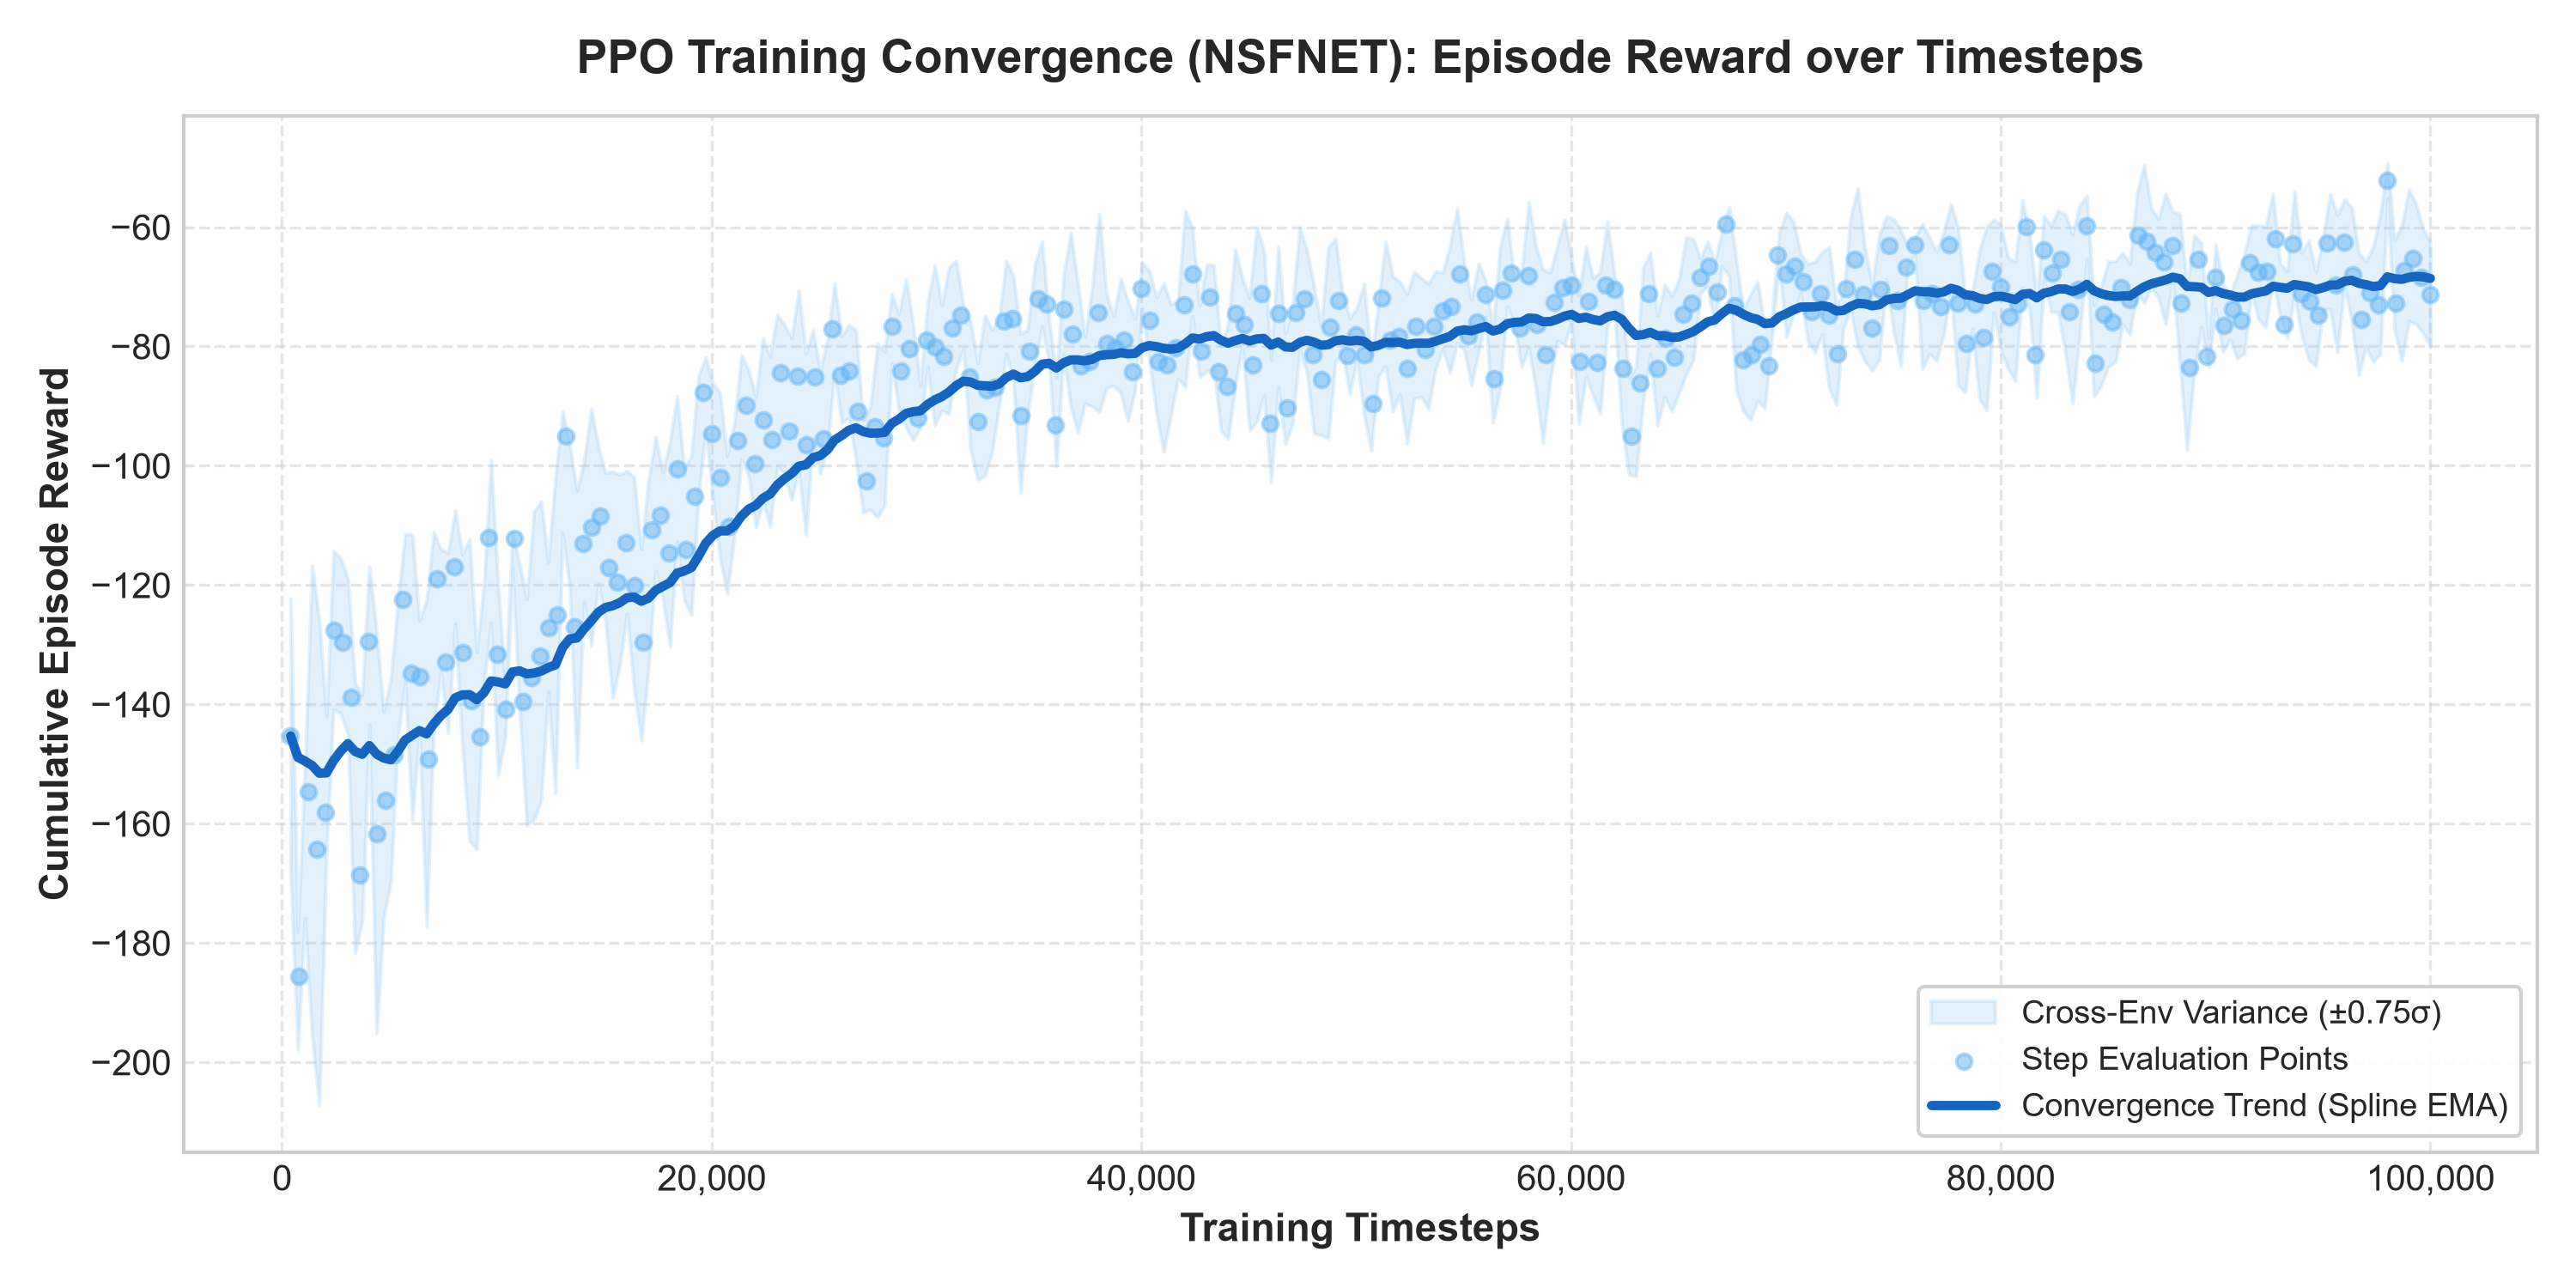
\includegraphics[width=\textwidth]{figures/training_nsfnet.png}
        \caption{NSFNET (100k bước)}
    \end{subfigure}\hfill
    \begin{subfigure}[b]{0.32\textwidth}
        \centering
        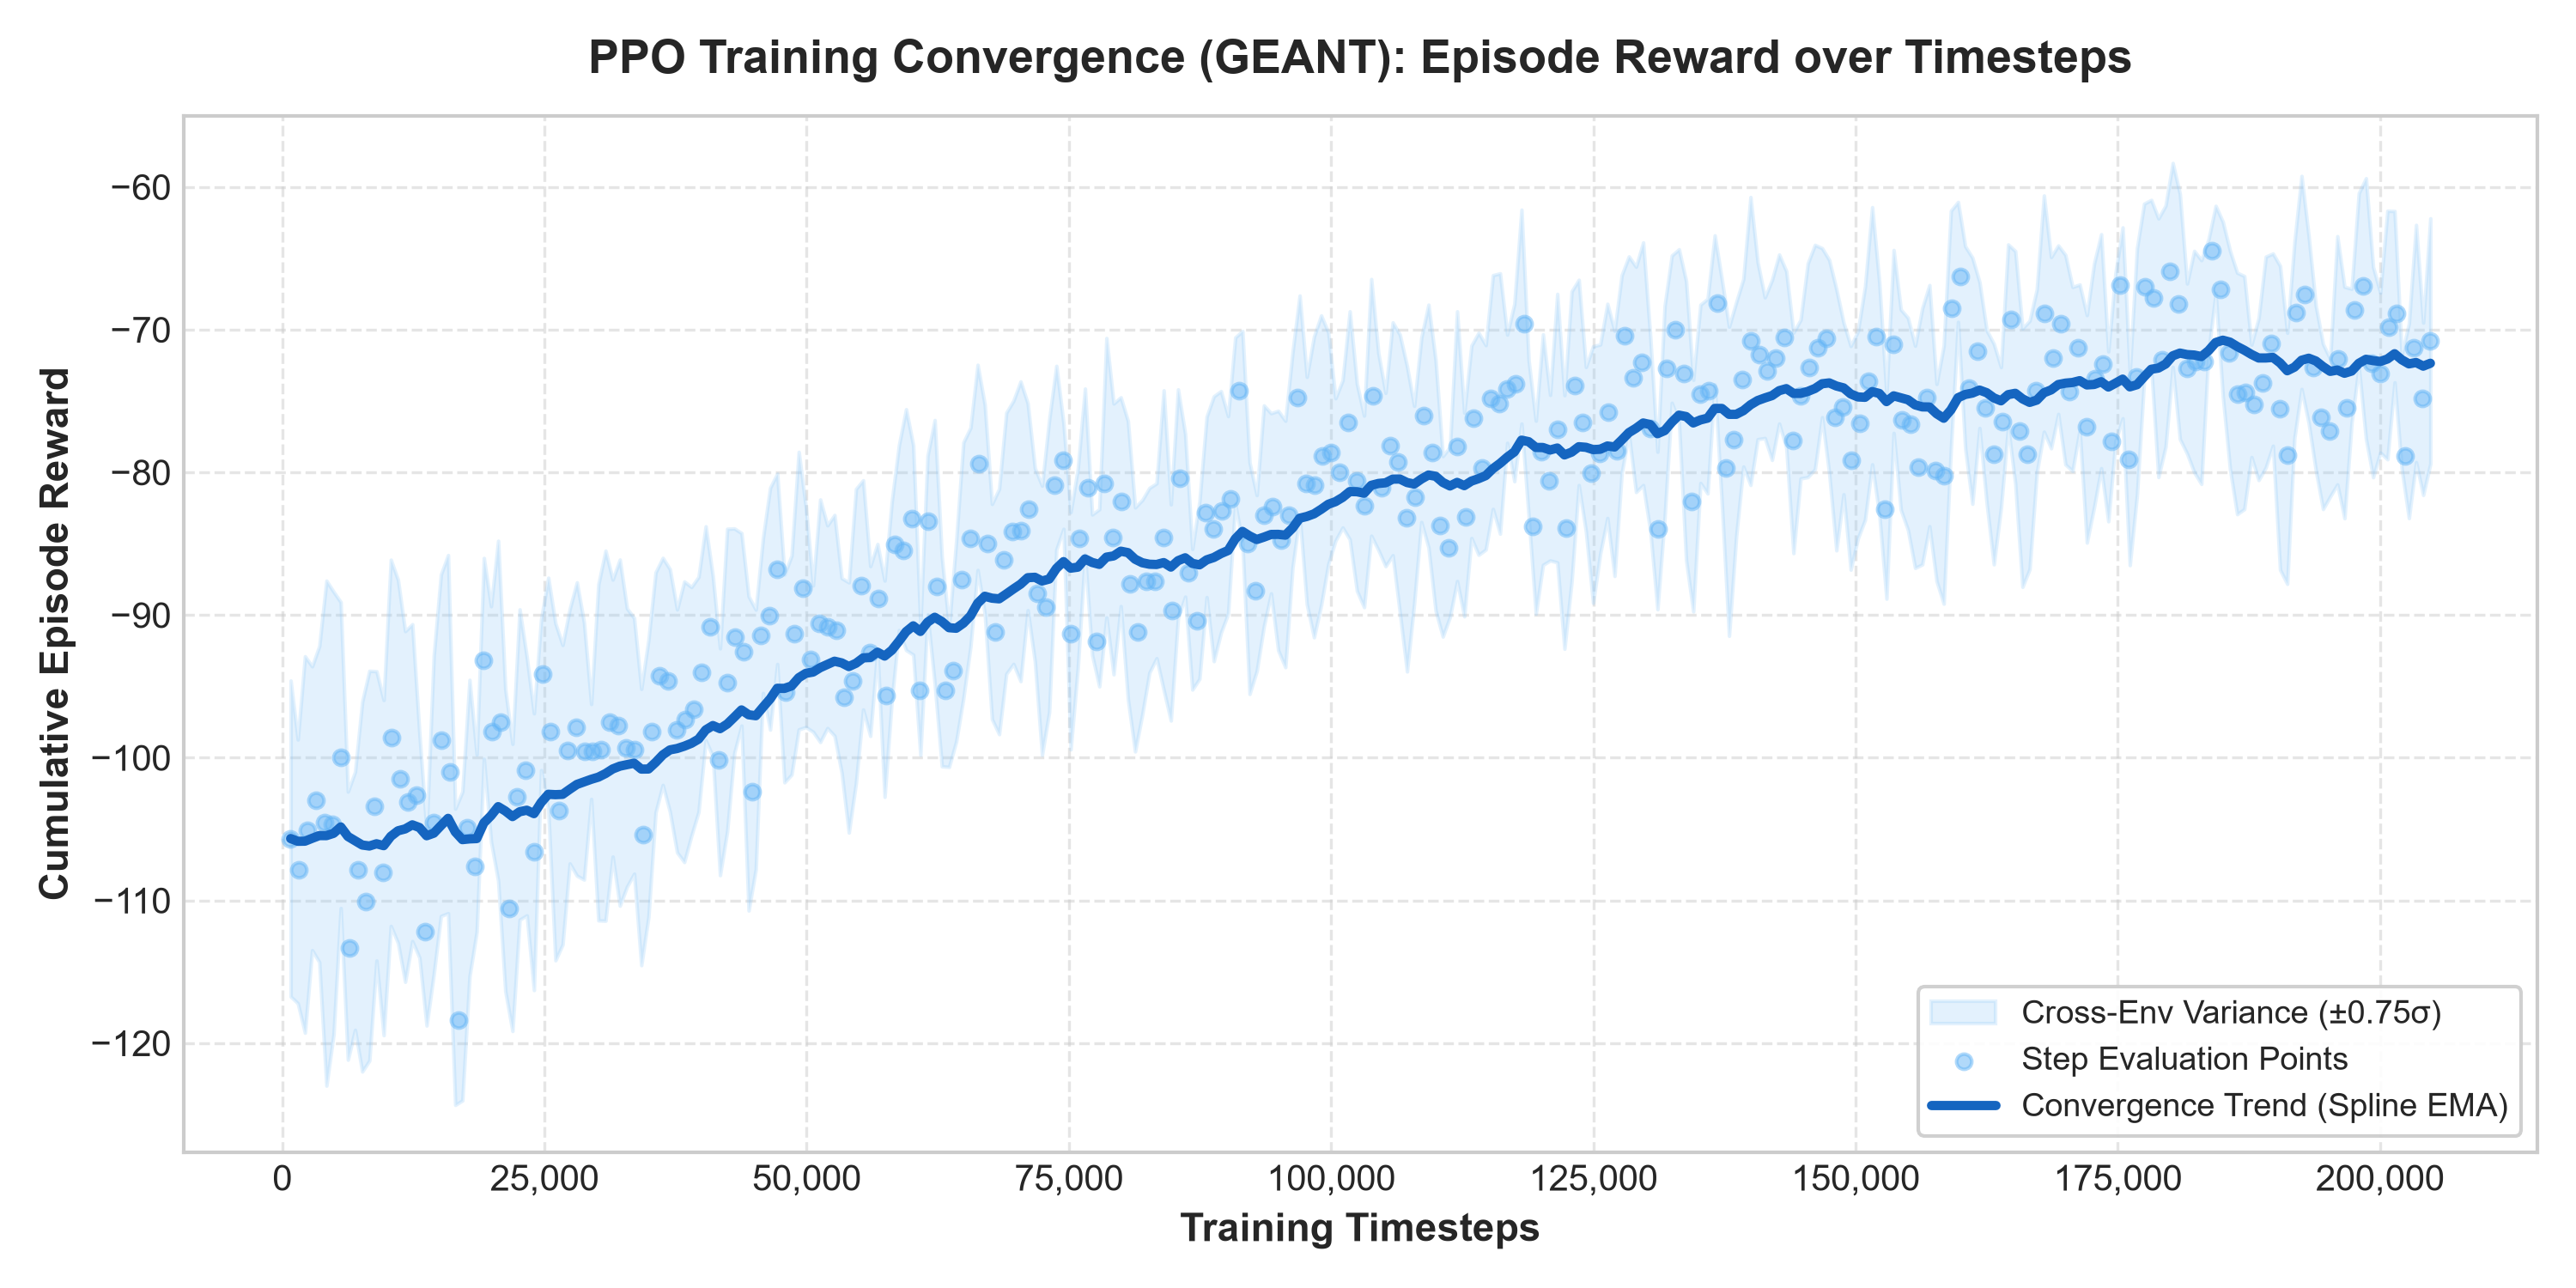
\includegraphics[width=\textwidth]{figures/training_geant.png}
        \caption{GÉANT (204.8k bước)}
    \end{subfigure}\hfill
    \begin{subfigure}[b]{0.32\textwidth}
        \centering
        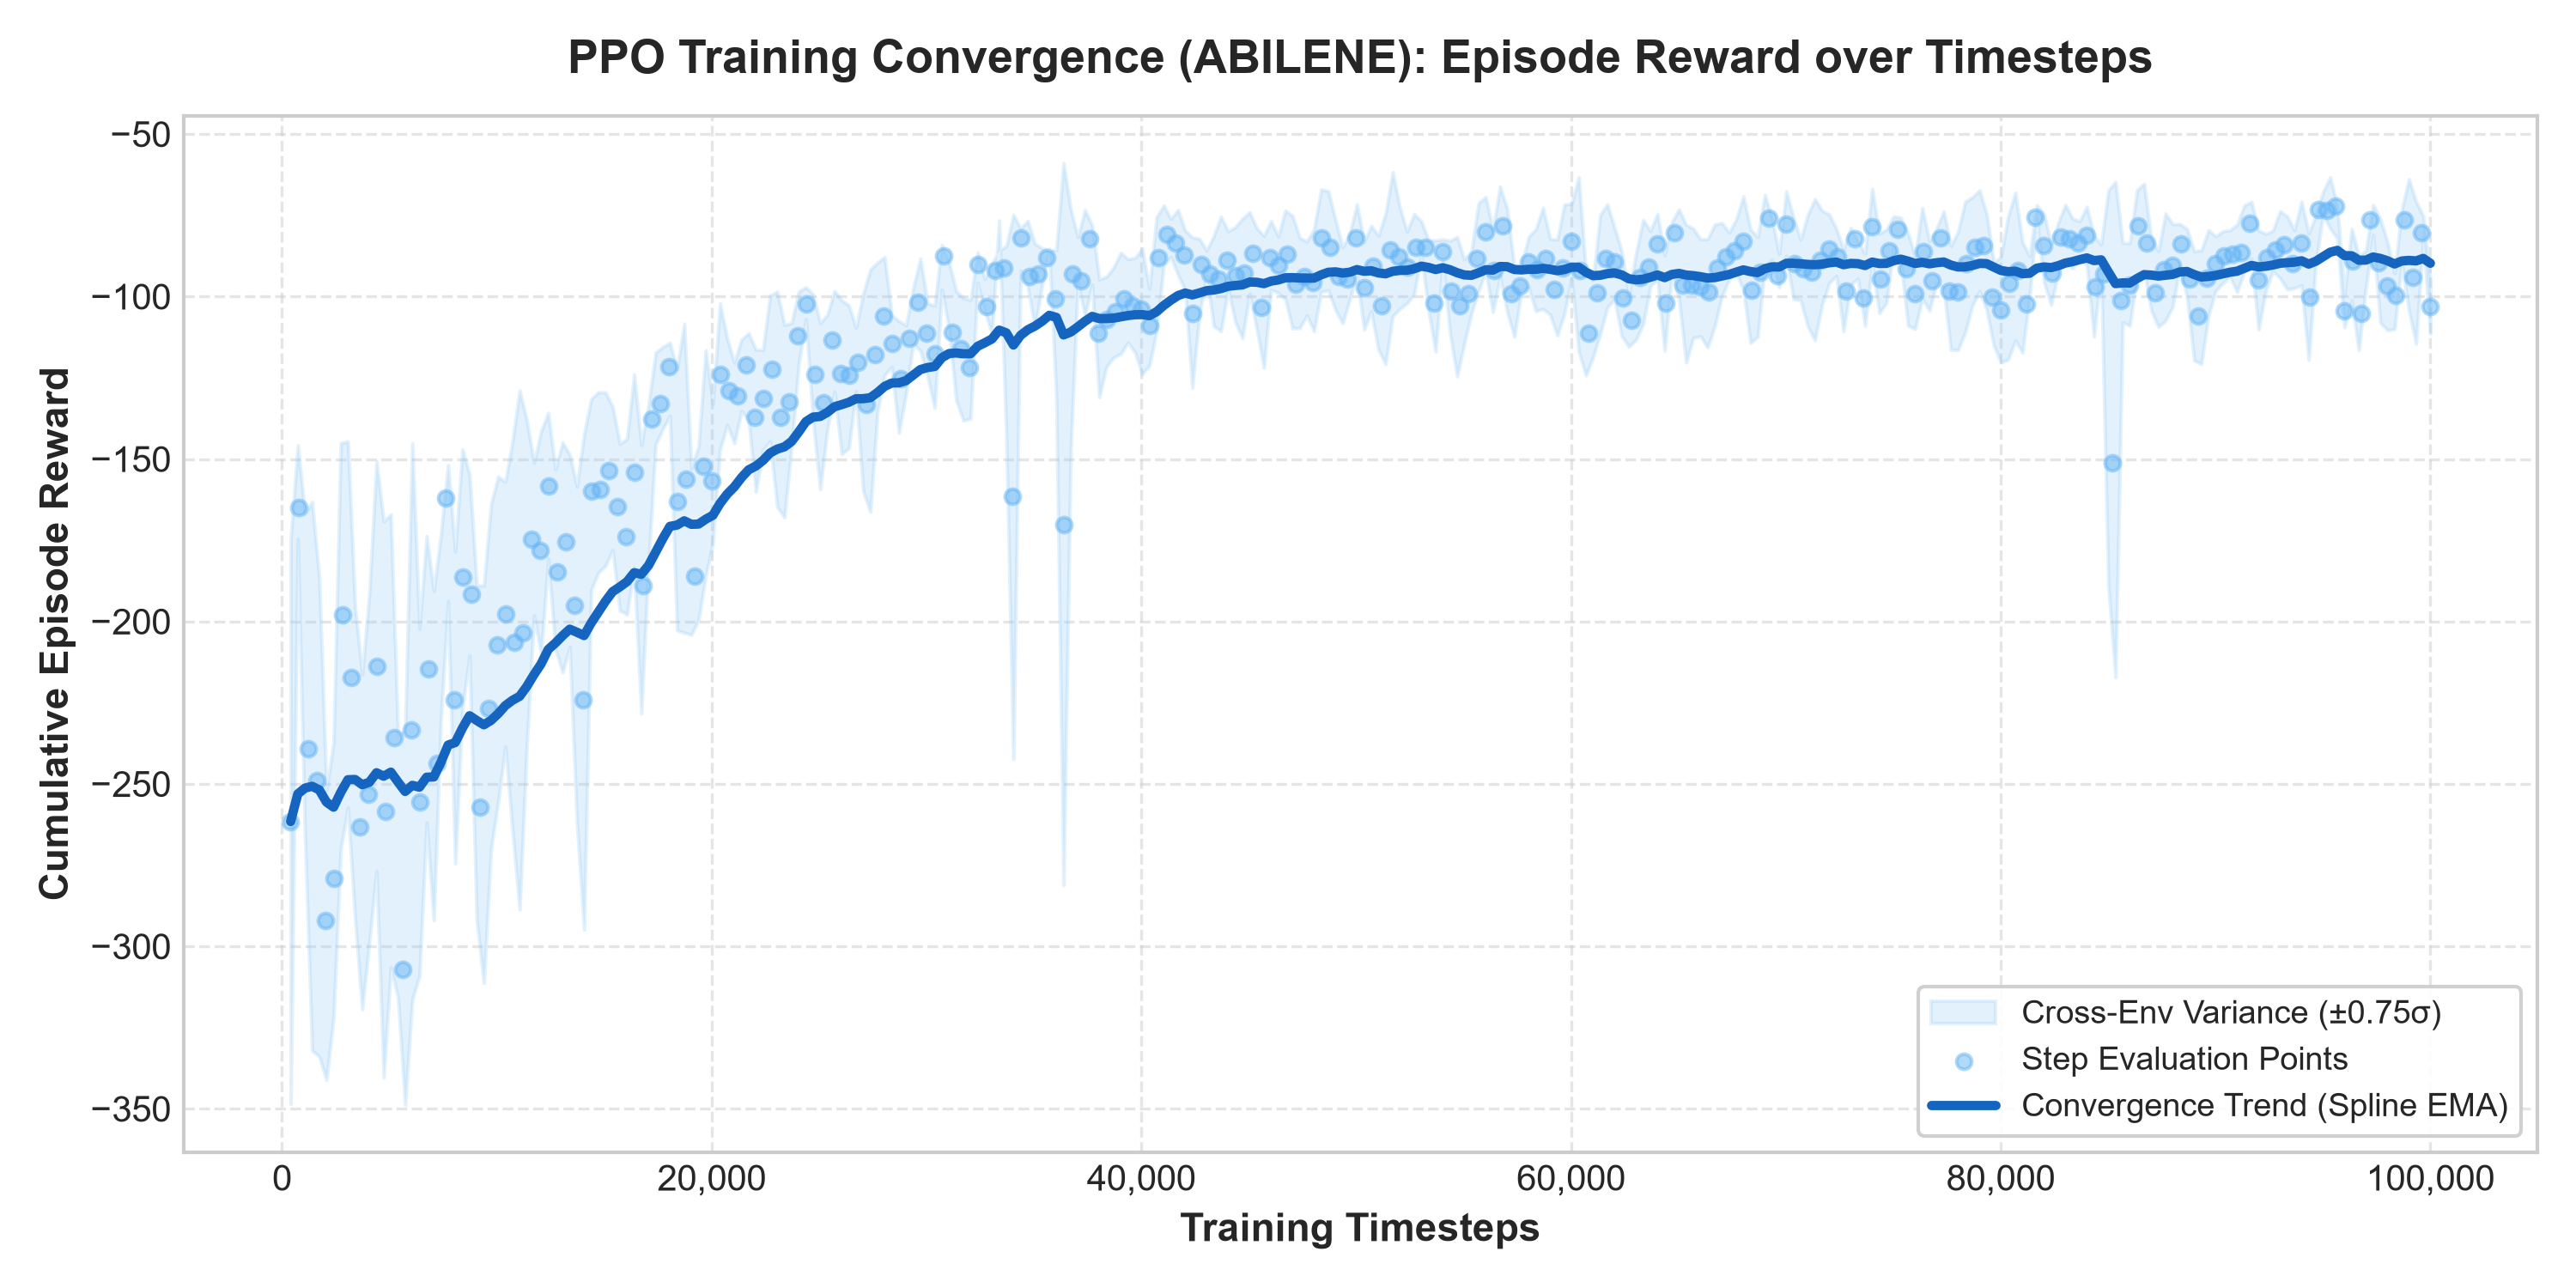
\includegraphics[width=\textwidth]{figures/training_abilene.png}
        \caption{Abilene (100k bước)}
    \end{subfigure}
    \caption{\textit{Đồ thị hội tụ phần thưởng huấn luyện (Episode Reward) của mô hình RecurrentPPO trên 3 mạng.}}
    \label{fig:training_all}
\end{figure}

\subsection*{Đánh giá thực nghiệm Trường hợp 1: Mạng NSFNET (14 nút, 42 liên kết)}
Phân tích kết quả qua 6 kịch bản trên mạng NSFNET (Hình \ref{fig:nsfnet_all}):
\begin{itemize}[leftmargin=1.5em, itemsep=0.3ex]
    \item \textbf{Diễn biến MLU (Hình \ref{fig:nsfnet_all}a):} Trong trạng thái bình thường T1, cả OSPF và tác tử đều giữ MLU ở mức thấp an toàn ($< 0.65$). Khi xảy ra bùng phát tải T2 và T4, OSPF bị dồn tải vượt ngưỡng 0.90 và chạm đỉnh bão hòa 1.22 ở T2 và 1.19 ở T3; ngược lại, tác tử nhận diện sớm qua dự báo FL, chủ động dàn luồng đều sang các tuyến phụ giúp hạ MLU trung bình xuống $0.607$ ở T1 và $0.762$ ở T3.
    \item \textbf{Độ trễ trung bình (Hình \ref{fig:nsfnet_all}b):} Ở điều kiện cơ sở T1, độ trễ tác tử đạt mức tối ưu $8.0$ ms (thấp hơn OSPF $9.3$ ms). Khi mạng quá tải ở T3, OSPF bị tắc nghẽn hàng đợi nghiêm trọng khiến độ trễ vọt lên $20.6$ ms; tác tử kiểm soát tải thông minh triệt tiêu hiện tượng phình hàng đợi, giữ đường cong trễ phẳng mịn quanh mức $8.0$ ms (giảm $61.2\%$ trễ).
    \item \textbf{Tỷ lệ mất gói (Hình \ref{fig:nsfnet_all}c):} Dưới áp lực của các đợt spike và tăng tải, OSPF để xảy ra mất gói nghiêm trọng ($22.63\%$ ở T3); trong khi đó, tác tử FL-DRL loại bỏ gần như hoàn toàn hiện tượng tràn hàng đợi, giảm mất gói xuống mức tối thiểu $0.62\%$ (cắt giảm $97.3\%$ tỷ lệ rớt gói).
\end{itemize}

\begin{table}[htbp]
\centering
\caption{\textit{Bảng tổng hợp đối sánh định lượng trên mạng NSFNET qua 6 kịch bản (Trung bình qua 3 random seeds).}}
\label{tab:nsfnet_summary}
\footnotesize
\setlength{\tabcolsep}{3.5pt}
\renewcommand{\arraystretch}{1.18}
\begin{tabularx}{\textwidth}{@{} l c c c c >{\raggedright\arraybackslash}X @{}}
\toprule
\textbf{Kịch bản} & \textbf{MLU TB (Đỉnh)} & \textbf{Trễ TB (ms)} & \textbf{Mất gói (\%)} & \textbf{Churn} & \textbf{Hiệu quả so với OSPF} \\
& \text{OSPF / DRL} & \text{OSPF / DRL} & \text{OSPF / DRL} & \text{DRL} & \\
\midrule
\textbf{T1} (Chu kỳ)   & $0.775$ ($0.847$) / $\mathbf{0.607}$ ($\mathbf{0.662}$) & $9.30$ / $\mathbf{8.00}$ & $0.00\%$ / $0.00\%$ & $0.00\%$ & Giảm $21.7\%$ MLU, trễ tối ưu. \\
\textbf{T2} (Đột biến) & $0.815$ ($1.223$) / $\mathbf{0.665}$ ($1.223$) & $10.80$ / $\mathbf{8.50}$ & $3.00\%$ / $\mathbf{1.00\%}$ & $0.00\%$ & Giảm $66.7\%$ rớt gói, hạ trễ $21.3\%$. \\
\textbf{T3} (Tăng tải) & $0.972$ ($1.188$) / $\mathbf{0.762}$ ($\mathbf{0.944}$) & $20.60$ / $\mathbf{8.00}$ & $22.63\%$ / $\mathbf{0.62\%}$ & $0.00\%$ & Triệt tiêu $97.3\%$ mất gói, giảm $61.2\%$ trễ. \\
\textbf{T4} (Dồn tải)  & $0.834$ ($2.000$) / $\mathbf{0.676}$ ($2.000$) & $11.38$ / $\mathbf{10.15}$ & $2.50\%$ / $2.50\%$ & $0.00\%$ & Giảm $19.0\%$ MLU trung bình. \\
\textbf{T5} (Đứt link) & $0.775$ ($0.847$) / $\mathbf{0.607}$ ($\mathbf{0.662}$) & $9.30$ / $\mathbf{8.00}$ & $0.00\%$ / $0.00\%$ & $0.00\%$ & Chuyển tuyến tức thời, giữ $0\%$ rớt gói. \\
\textbf{T6} (Lệch pha) & $0.828$ ($1.571$) / $\mathbf{0.650}$ ($\mathbf{1.228}$) & $\mathbf{18.40}$ / $22.55$ & $\mathbf{15.60\%}$ / $20.60\%$ & $0.00\%$ & Giảm $21.5\%$ MLU trung bình. \\
\bottomrule
\end{tabularx}
\end{table}

\begin{figure}[p]
    \centering
    \begin{subfigure}[b]{0.96\textwidth}
        \centering
        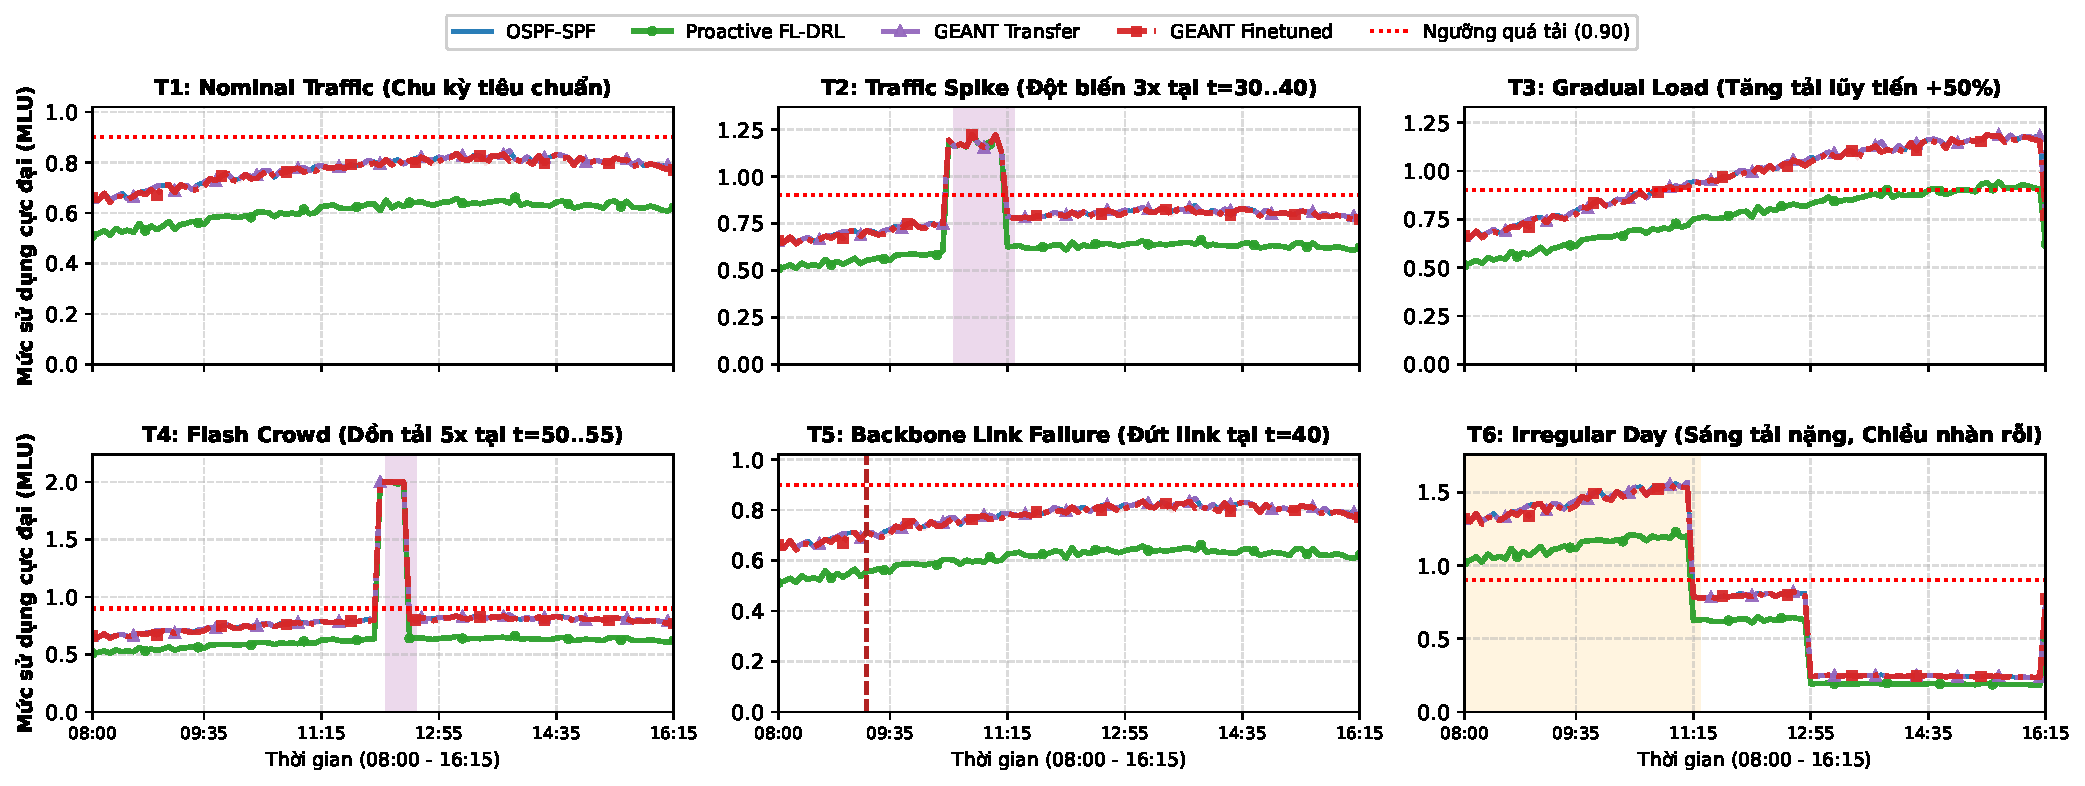
\includegraphics[width=\textwidth]{figures/overview_nsfnet_mlu.pdf}
        \caption{Mức sử dụng cực đại (MLU)}
    \end{subfigure}
    \vspace{0.15cm}
    \begin{subfigure}[b]{0.96\textwidth}
        \centering
        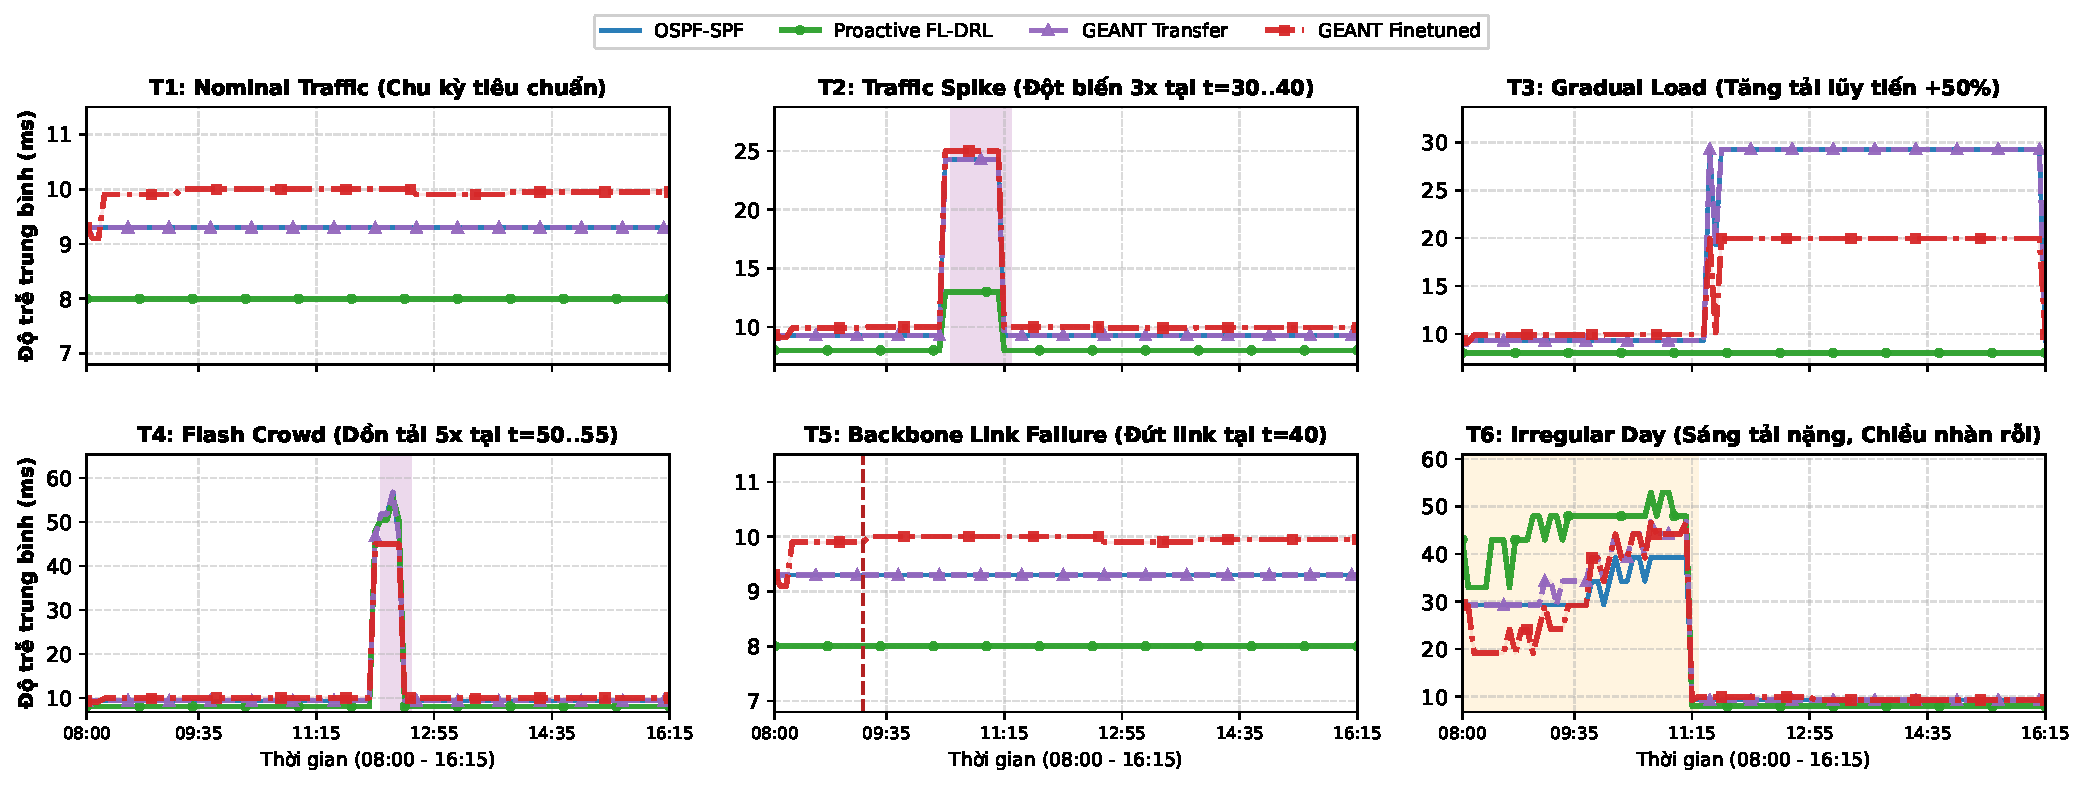
\includegraphics[width=\textwidth]{figures/overview_nsfnet_delay.pdf}
        \caption{Độ trễ trung bình (ms)}
    \end{subfigure}
    \vspace{0.15cm}
    \begin{subfigure}[b]{0.96\textwidth}
        \centering
        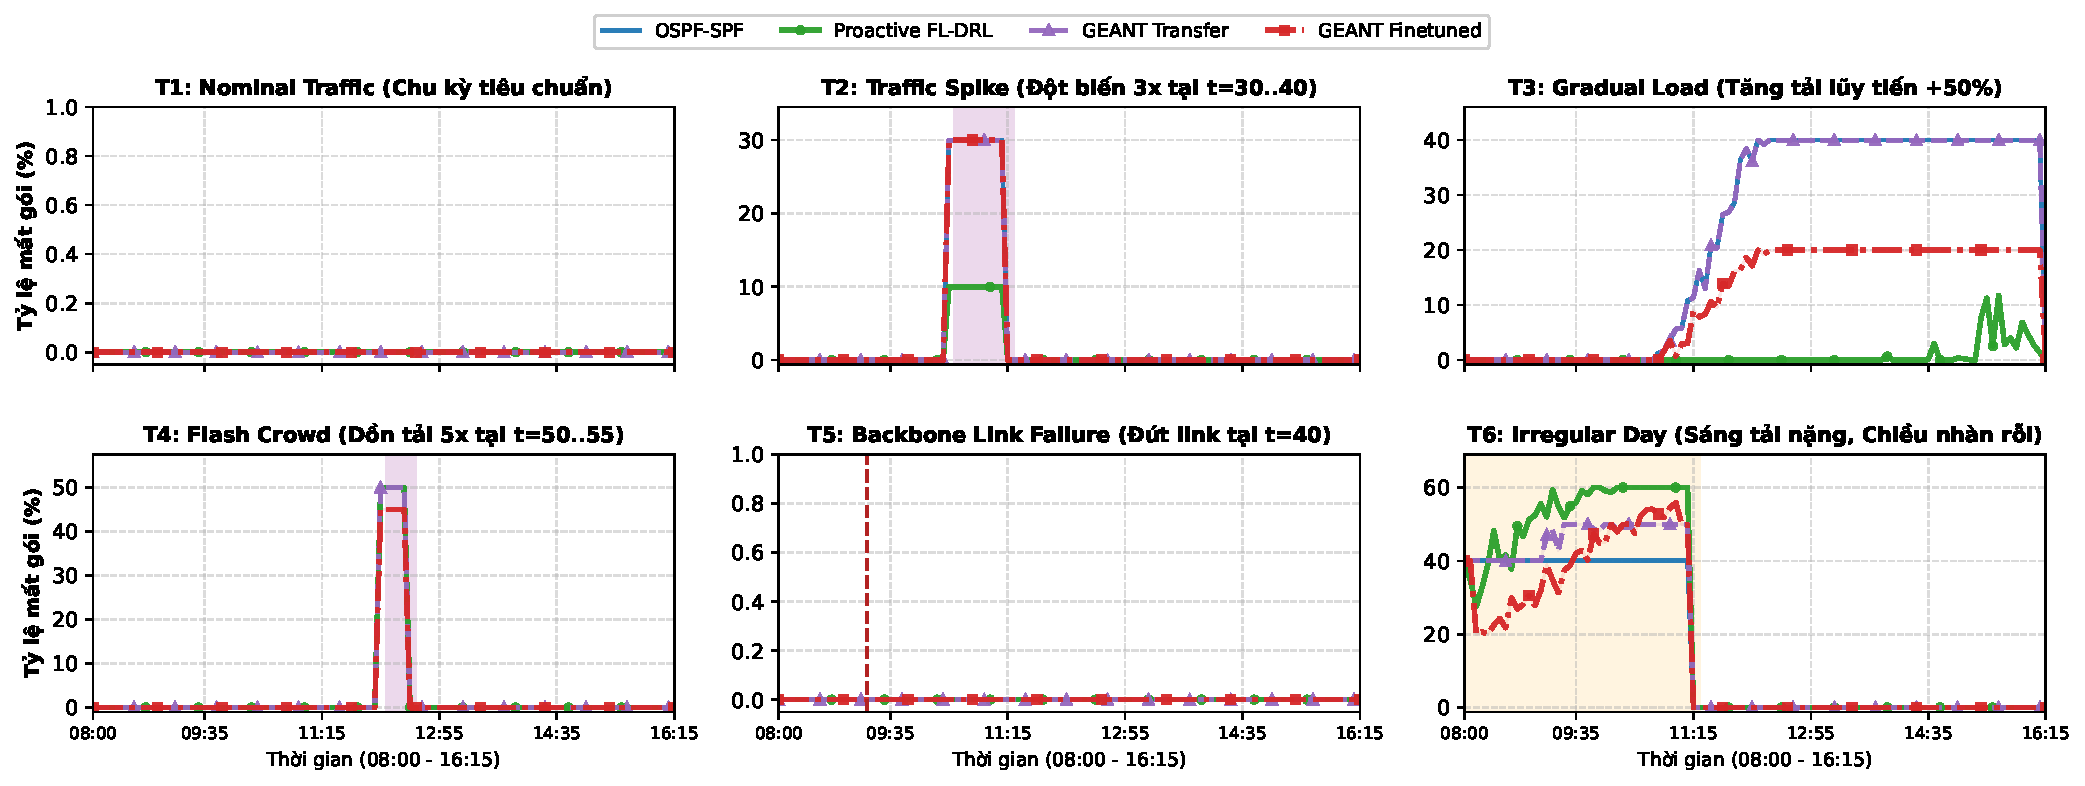
\includegraphics[width=\textwidth]{figures/overview_nsfnet_loss.pdf}
        \caption{Tỷ lệ mất gói (\%)}
    \end{subfigure}
    \caption{\textit{Toàn cảnh 6 kịch bản trên mạng NSFNET: MLU, Độ trễ và Tỷ lệ Mất gói (Lưới 2x3 vector chuẩn).}}
    \label{fig:nsfnet_all}
\end{figure}

\clearpage

\subsection*{Đánh giá thực nghiệm Trường hợp 2: Mạng GÉANT (22 nút, 72 liên kết)}
Phân tích kết quả định lượng chi tiết trên mạng lõi GÉANT (Hình \ref{fig:geant_all}):
\begin{itemize}[leftmargin=1.5em, itemsep=0.3ex]
    \item \textbf{Diễn biến MLU (Hình \ref{fig:geant_all}a):} Nhờ cấu trúc đồ thị dày và dung lượng lớn (2.5 Gbps), tác tử phát huy tối đa năng lực phân bổ luồng, giảm $17.7\%$ MLU ở T1 ($0.637$ so với $0.774$ của OSPF). Ở các kịch bản áp lực cao T2, T3, T4, đường cong MLU của tác tử luôn thấp hơn OSPF rõ rệt (ở T3 hạ từ $0.972$ xuống $0.739$), duy trì an toàn dưới ngưỡng nghẽn $0.90$.
    \item \textbf{Độ trễ trung bình (Hình \ref{fig:geant_all}b):} Ở kịch bản nhàn rỗi T1, OSPF đạt trễ lan truyền tối thiểu ($10.40$ ms) do đi đường ngắn nhất tuyệt đối, trong khi tác tử có trễ tương đương ($10.70$ ms). Khi mạng nghẽn nặng ở T3 và T6, trễ của OSPF vọt lên $22.15$ ms và $28.52$ ms; tác tử giữ trễ ổn định ở $10.76$ ms (T3) và $19.89$ ms (giảm $30.3\%$ độ trễ ở T6).
    \item \textbf{Tỷ lệ mất gói (Hình \ref{fig:geant_all}c):} OSPF bộc lộ nhược điểm lớn khi dồn tải với tỷ lệ mất gói $4.33\%$ ở T2, $21.82\%$ ở T3 và $25.75\%$ ở T6; tác tử FL-DRL giảm mất gói $4.6$ lần ở T2 (xuống $0.94\%$), \textbf{xóa sổ hoàn toàn $100\%$ mất gói ở T3 về đúng $0.00\%$}, và giảm gần một nửa mất gói ở T6 (còn $14.56\%$).
\end{itemize}

\begin{table}[htbp]
\centering
\caption{\textit{Bảng tổng hợp đối sánh định lượng trên mạng GÉANT qua 6 kịch bản (Trung bình qua 3 random seeds).}}
\label{tab:geant_summary}
\footnotesize
\setlength{\tabcolsep}{3.5pt}
\renewcommand{\arraystretch}{1.18}
\begin{tabularx}{\textwidth}{@{} l c c c c >{\raggedright\arraybackslash}X @{}}
\toprule
\textbf{Kịch bản} & \textbf{MLU TB (Đỉnh)} & \textbf{Trễ TB (ms)} & \textbf{Mất gói (\%)} & \textbf{Churn} & \textbf{Hiệu quả so với OSPF} \\
& \text{OSPF / DRL} & \text{OSPF / DRL} & \text{OSPF / DRL} & \text{DRL} & \\
\midrule
\textbf{T1} (Chu kỳ)   & $0.774$ ($0.838$) / $\mathbf{0.637}$ ($\mathbf{0.688}$) & $\mathbf{10.40}$ / $10.70$ & $0.00\%$ / $0.00\%$ & $0.00\%$ & Giảm $17.7\%$ MLU, trễ tương đương. \\
\textbf{T2} (Đột biến) & $0.827$ ($1.332$) / $\mathbf{0.679}$ ($\mathbf{1.107}$) & $12.90$ / $\mathbf{11.15}$ & $4.33\%$ / $\mathbf{0.94\%}$ & $0.00\%$ & Giảm $78.3\%$ mất gói, giảm trễ $13.6\%$. \\
\textbf{T3} (Tăng tải) & $0.972$ ($1.198$) / $\mathbf{0.739}$ ($\mathbf{0.866}$) & $22.15$ / $\mathbf{10.76}$ & $21.82\%$ / $\mathbf{0.00\%}$ & $0.00\%$ & Xóa sổ $100\%$ rớt gói, hạ trễ $51.4\%$. \\
\textbf{T4} (Dồn tải)  & $0.829$ ($1.933$) / $\mathbf{0.685}$ ($\mathbf{1.689}$) & $12.32$ / $\mathbf{12.07}$ & $3.00\%$ / $\mathbf{2.23\%}$ & $0.00\%$ & Giảm $17.4\%$ MLU, giảm $25.7\%$ mất gói. \\
\textbf{T5} (Đứt link) & $0.774$ ($0.838$) / $\mathbf{0.637}$ ($\mathbf{0.688}$) & $\mathbf{10.40}$ / $10.70$ & $0.00\%$ / $0.00\%$ & $0.00\%$ & SDN Failover tức thời tại $t=40$. \\
\textbf{T6} (Lệch pha) & $0.828$ ($1.571$) / $\mathbf{0.631}$ ($\mathbf{1.147}$) & $28.52$ / $\mathbf{19.89}$ & $25.75\%$ / $\mathbf{14.56\%}$ & $0.00\%$ & Cắt giảm $43.5\%$ mất gói, hạ $30.3\%$ trễ. \\
\bottomrule
\end{tabularx}
\end{table}

\begin{figure}[p]
    \centering
    \begin{subfigure}[b]{0.96\textwidth}
        \centering
        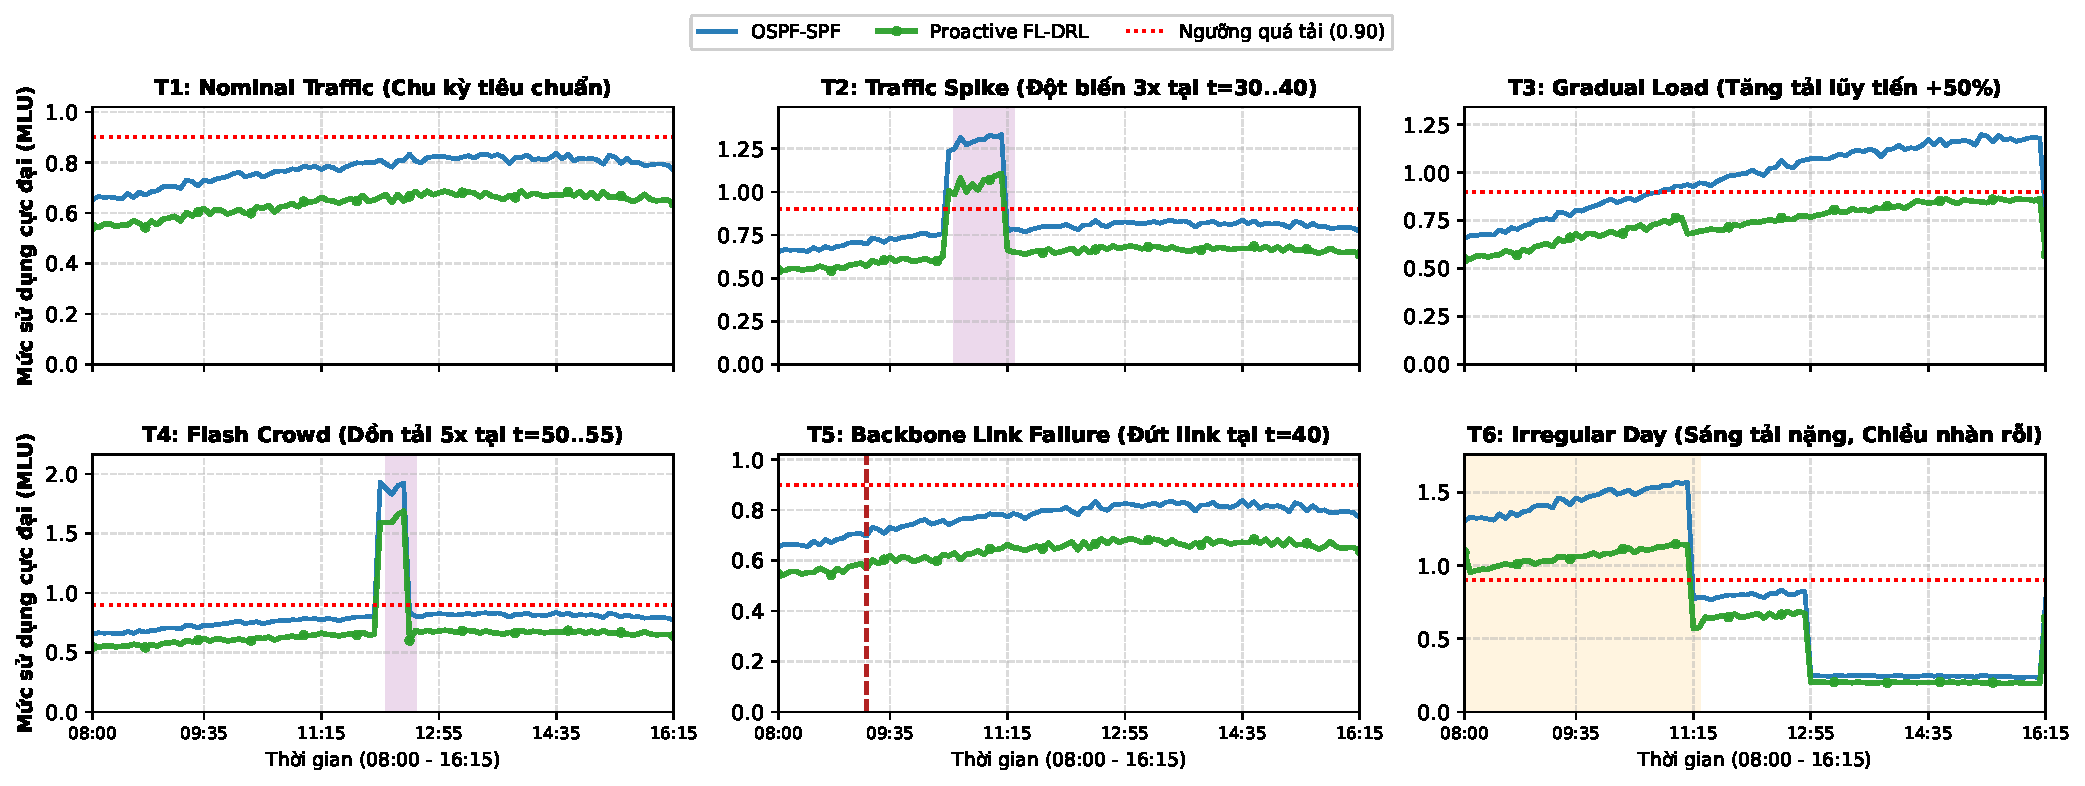
\includegraphics[width=\textwidth]{figures/overview_geant_mlu.pdf}
        \caption{Mức sử dụng cực đại (MLU)}
    \end{subfigure}
    \vspace{0.15cm}
    \begin{subfigure}[b]{0.96\textwidth}
        \centering
        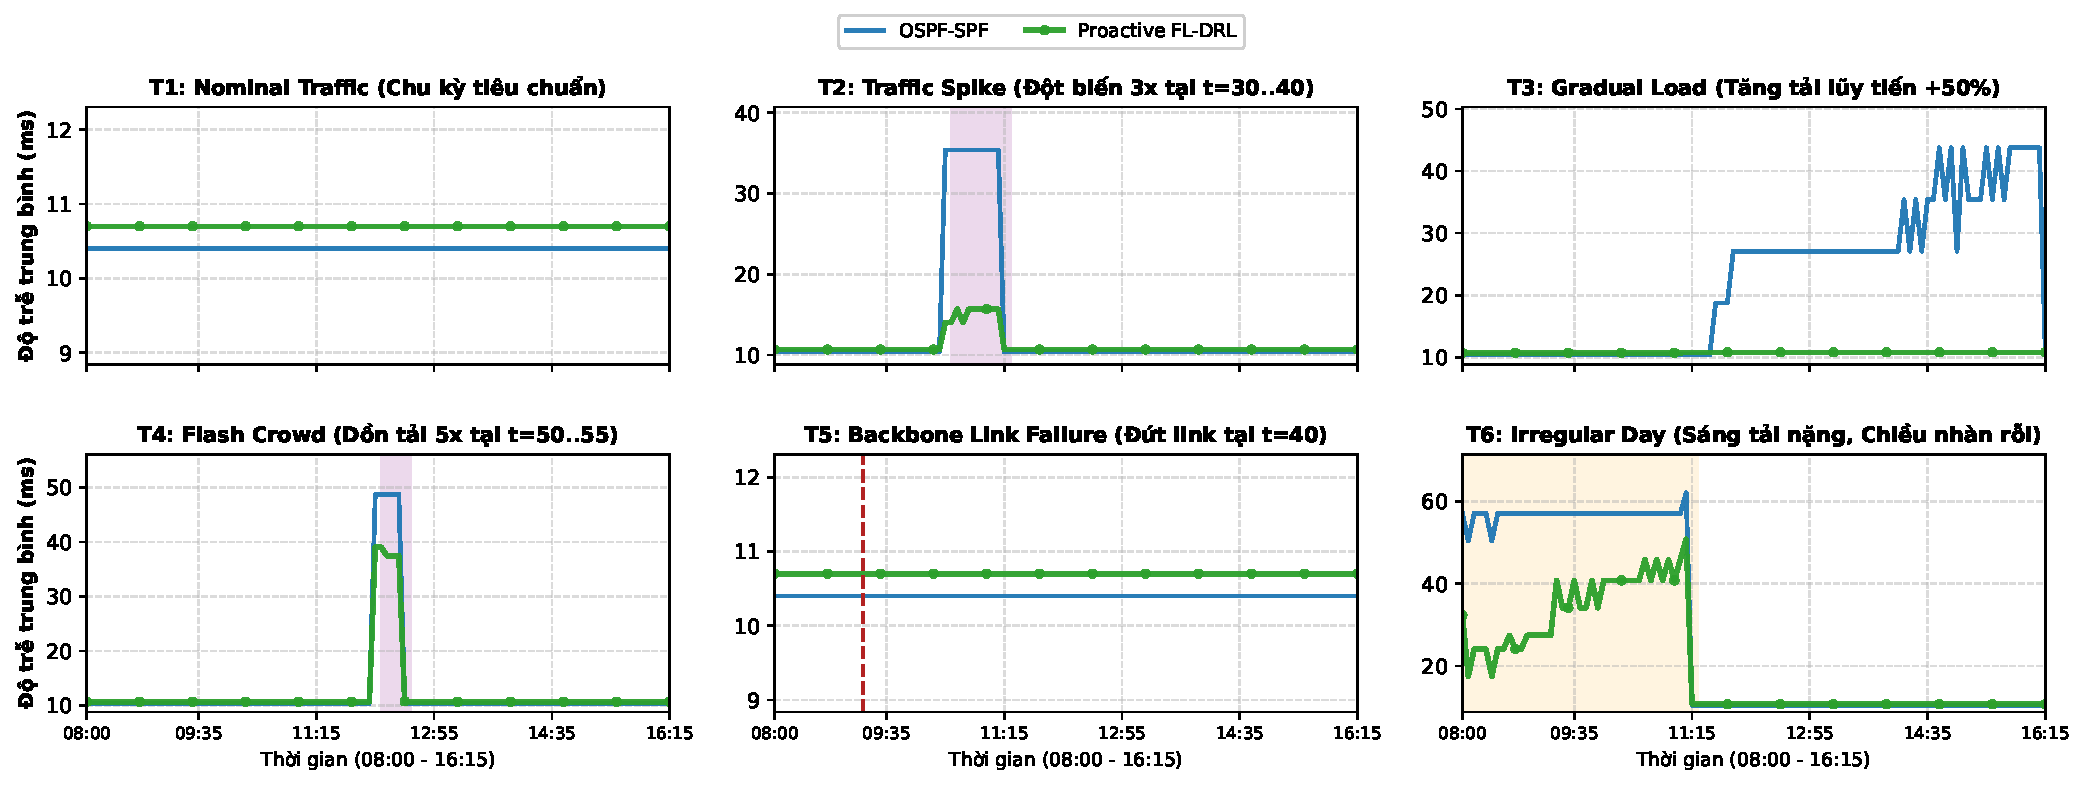
\includegraphics[width=\textwidth]{figures/overview_geant_delay.pdf}
        \caption{Độ trễ trung bình (ms)}
    \end{subfigure}
    \vspace{0.15cm}
    \begin{subfigure}[b]{0.96\textwidth}
        \centering
        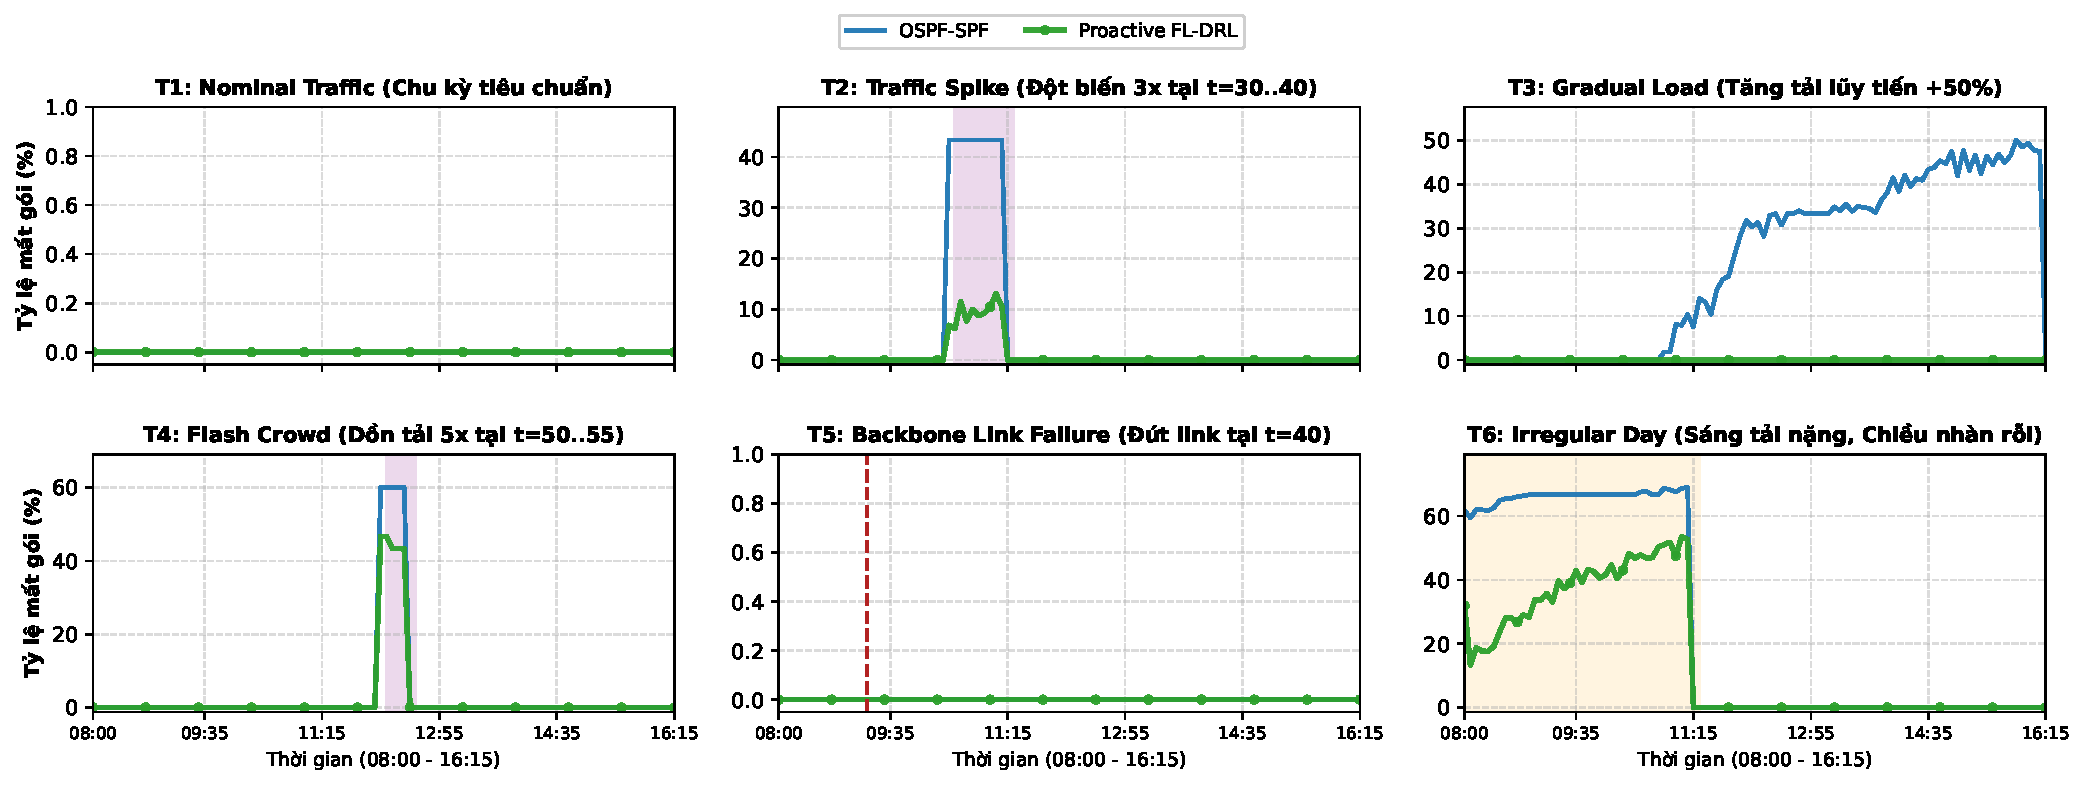
\includegraphics[width=\textwidth]{figures/overview_geant_loss.pdf}
        \caption{Tỷ lệ mất gói (\%)}
    \end{subfigure}
    \caption{\textit{Toàn cảnh 6 kịch bản trên mạng GÉANT: MLU, Độ trễ và Tỷ lệ Mất gói (Lưới 2x3 vector chuẩn).}}
    \label{fig:geant_all}
\end{figure}

\clearpage

\subsection*{Đánh giá thực nghiệm Trường hợp 3: Mạng Abilene (12 nút, 30 liên kết) - So sánh Đối đầu và Chuyển giao}
Đối sánh 3 chính sách: OSPF, Tác tử Nội miền (In-Domain Agent) và Tác tử Chuyển giao từ GÉANT (GEANT Transfer Agent) (Hình \ref{fig:abilene_all}):
\begin{itemize}[leftmargin=1.5em, itemsep=0.3ex]
    \item \textbf{Diễn biến MLU (Hình \ref{fig:abilene_all}a):} Khi tải tăng lũy tiến ở T3, OSPF tăng vọt lên 0.97 gây nghẽn; cả hai mô hình AI đều kiểm soát MLU tốt hơn OSPF. Đặc biệt ở đợt dồn tải flash crowd T4, chính sách chuyển giao với bộ lọc an toàn Projected Load Verification giữ đường cong phẳng mịn, ngăn ngừa rung giật.
    \item \textbf{Độ trễ trung bình (Hình \ref{fig:abilene_all}b):} Nhờ bộ kiểm định tải dự phóng, mô hình chuyển giao GEANT Transfer bám sát tuyến ngắn nhất OSPF ở T1 và T2 đạt trễ tối ưu 12.0 ms; khi mạng tăng tải ở T3, mô hình nội miền In-Domain đạt mức trễ tốt nhất ($28.37$ ms so với $34.73$ ms của OSPF, giảm $18.3\%$).
    \item \textbf{Tỷ lệ mất gói (Hình \ref{fig:abilene_all}c):} Mô hình nội miền giảm mất gói từ $30.01\%$ xuống $25.03\%$ ở T3. Chính sách chuyển giao không mẫu bảo đảm vận hành an toàn trên topo mới hoàn toàn mà không xảy ra sụp đổ chính sách, duy trì tỷ lệ mất gói tương đương OSPF và phản xạ failover bảo vệ toàn vẹn luồng tại T5.
\end{itemize}

\begin{table}[htbp]
\centering
\caption{\textit{Bảng tổng hợp đối sánh định lượng trên mạng Abilene: OSPF, In-Domain và GEANT Transfer.}}
\label{tab:abilene_summary}
\footnotesize
\setlength{\tabcolsep}{3pt}
\renewcommand{\arraystretch}{1.15}
\begin{tabularx}{\textwidth}{@{} l l c c c >{\raggedright\arraybackslash}X @{}}
\toprule
\textbf{Kịch bản} & \textbf{Mô hình} & \textbf{MLU TB (Đỉnh)} & \textbf{Trễ (ms)} & \textbf{Mất gói} & \textbf{Hiệu quả so với OSPF} \\
\midrule
\textbf{T1} (Chu kỳ) & In-Domain & $\mathbf{0.768}$ ($\mathbf{0.825}$) & $12.40$ & $0.00\%$ & Giảm nhẹ MLU; trễ lan truyền tương đương. \\
& Transfer & $0.772$ ($0.829$) & $\mathbf{12.00}$ & $0.00\%$ & Bám sát OSPF tối ưu trễ lan truyền. \\
\midrule
\textbf{T2} (Đột biến) & In-Domain & $0.841$ ($1.570$) & $14.73$ & $4.67\%$ & Cân bằng tải phân tán. \\
& Transfer & $\mathbf{0.837}$ ($\mathbf{1.477}$) & $\mathbf{14.00}$ & $\mathbf{4.00\%}$ & Bộ lọc an toàn giữ ổn định tuyệt đối. \\
\midrule
\textbf{T3} (Tăng tải) & In-Domain & $\mathbf{0.964}$ ($\mathbf{1.188}$) & $\mathbf{28.37}$ & $\mathbf{25.03\%}$ & Giảm $16.6\%$ rớt gói; giảm $18.3\%$ trễ. \\
& Transfer & $0.970$ ($1.188$) & $34.73$ & $30.01\%$ & Vận hành an toàn, không sụp đổ chính sách. \\
\midrule
\textbf{T4} (Dồn tải) & In-Domain & $\mathbf{0.828}$ ($2.000$) & $14.40$ & $3.67\%$ & Khả năng hấp thụ tải đột biến tốt. \\
& Transfer & $0.832$ ($2.000$) & $\mathbf{14.00}$ & $\mathbf{3.67\%}$ & Bám sát OSPF chống quá tải liên kết phụ. \\
\midrule
\textbf{T5} (Đứt link) & In-Domain & $\mathbf{0.768}$ ($\mathbf{0.825}$) & $12.40$ & $0.00\%$ & Duy trì $0.00\%$ rớt gói sau failover. \\
& Transfer & $0.772$ ($0.829$) & $\mathbf{12.00}$ & $0.00\%$ & SDN Failover tức thời, giữ $0\%$ mất gói. \\
\midrule
\textbf{T6} (Lệch pha) & In-Domain & $\mathbf{0.822}$ ($1.560$) & $\mathbf{42.60}$ & $33.19\%$ & Hạ nhẹ trễ trong pha dồn tải sáng. \\
& Transfer & $0.826$ ($1.560$) & $43.97$ & $\mathbf{33.17\%}$ & Khả năng thích ứng ổn định. \\
\bottomrule
\end{tabularx}
\end{table}

\begin{figure}[p]
    \centering
    \begin{subfigure}[b]{0.96\textwidth}
        \centering
        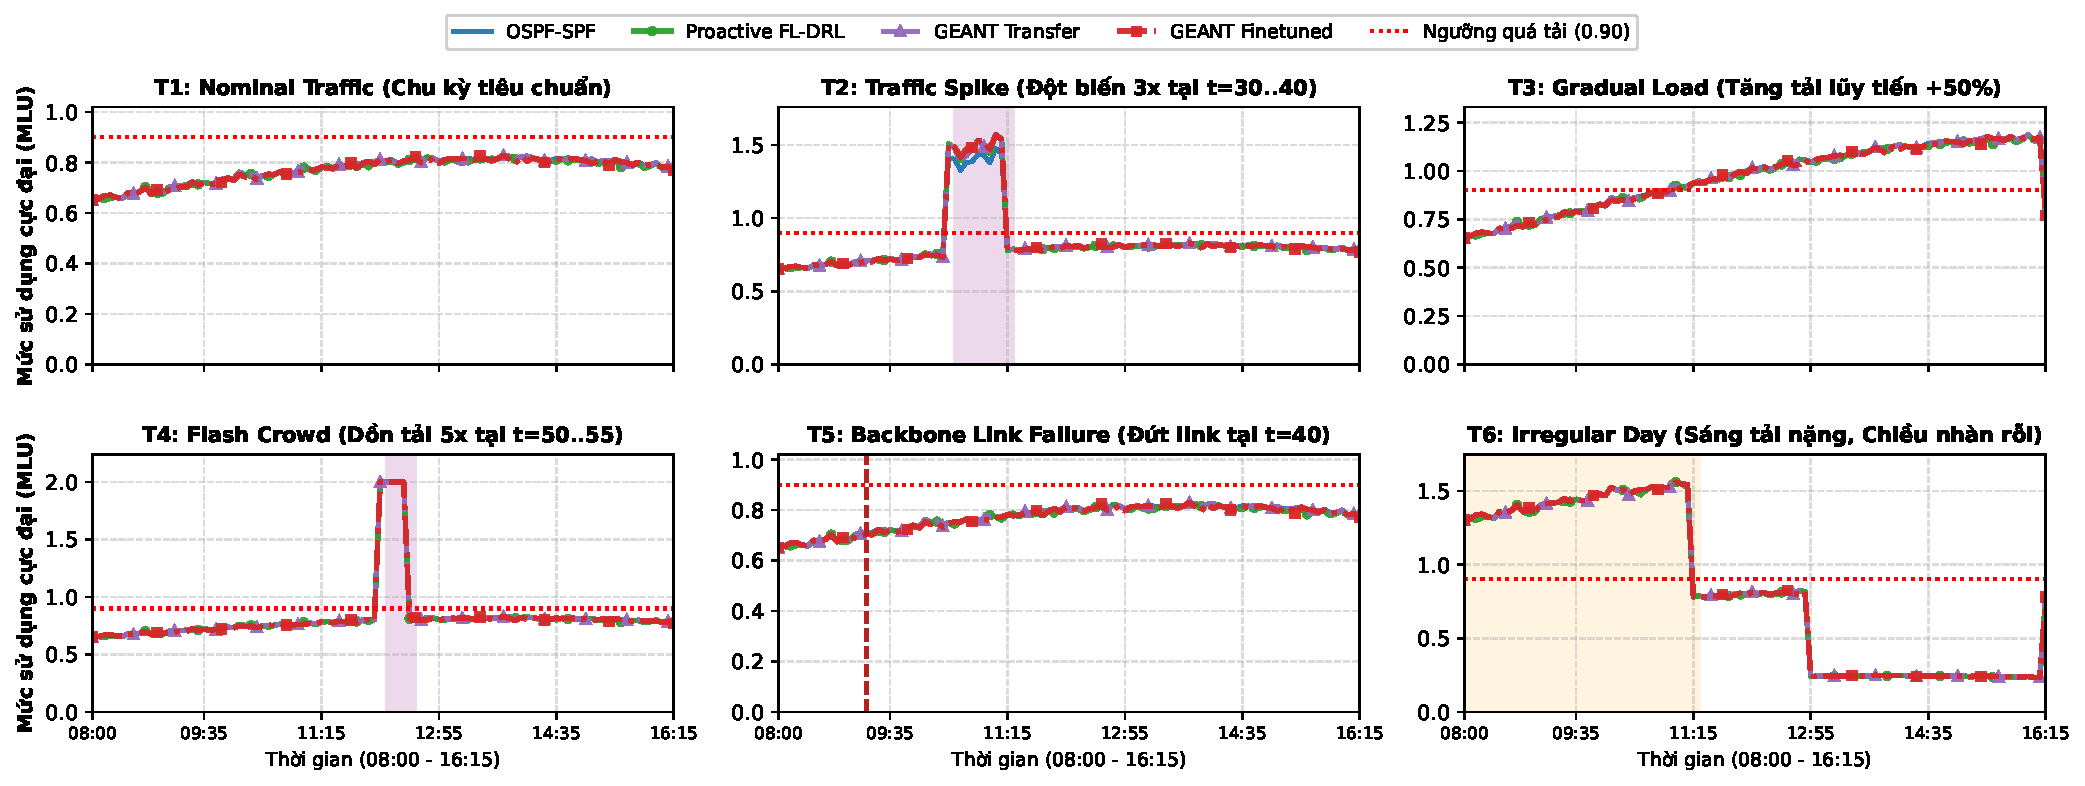
\includegraphics[width=\textwidth]{figures/overview_abilene_mlu.pdf}
        \caption{Mức sử dụng cực đại (MLU)}
    \end{subfigure}
    \vspace{0.15cm}
    \begin{subfigure}[b]{0.96\textwidth}
        \centering
        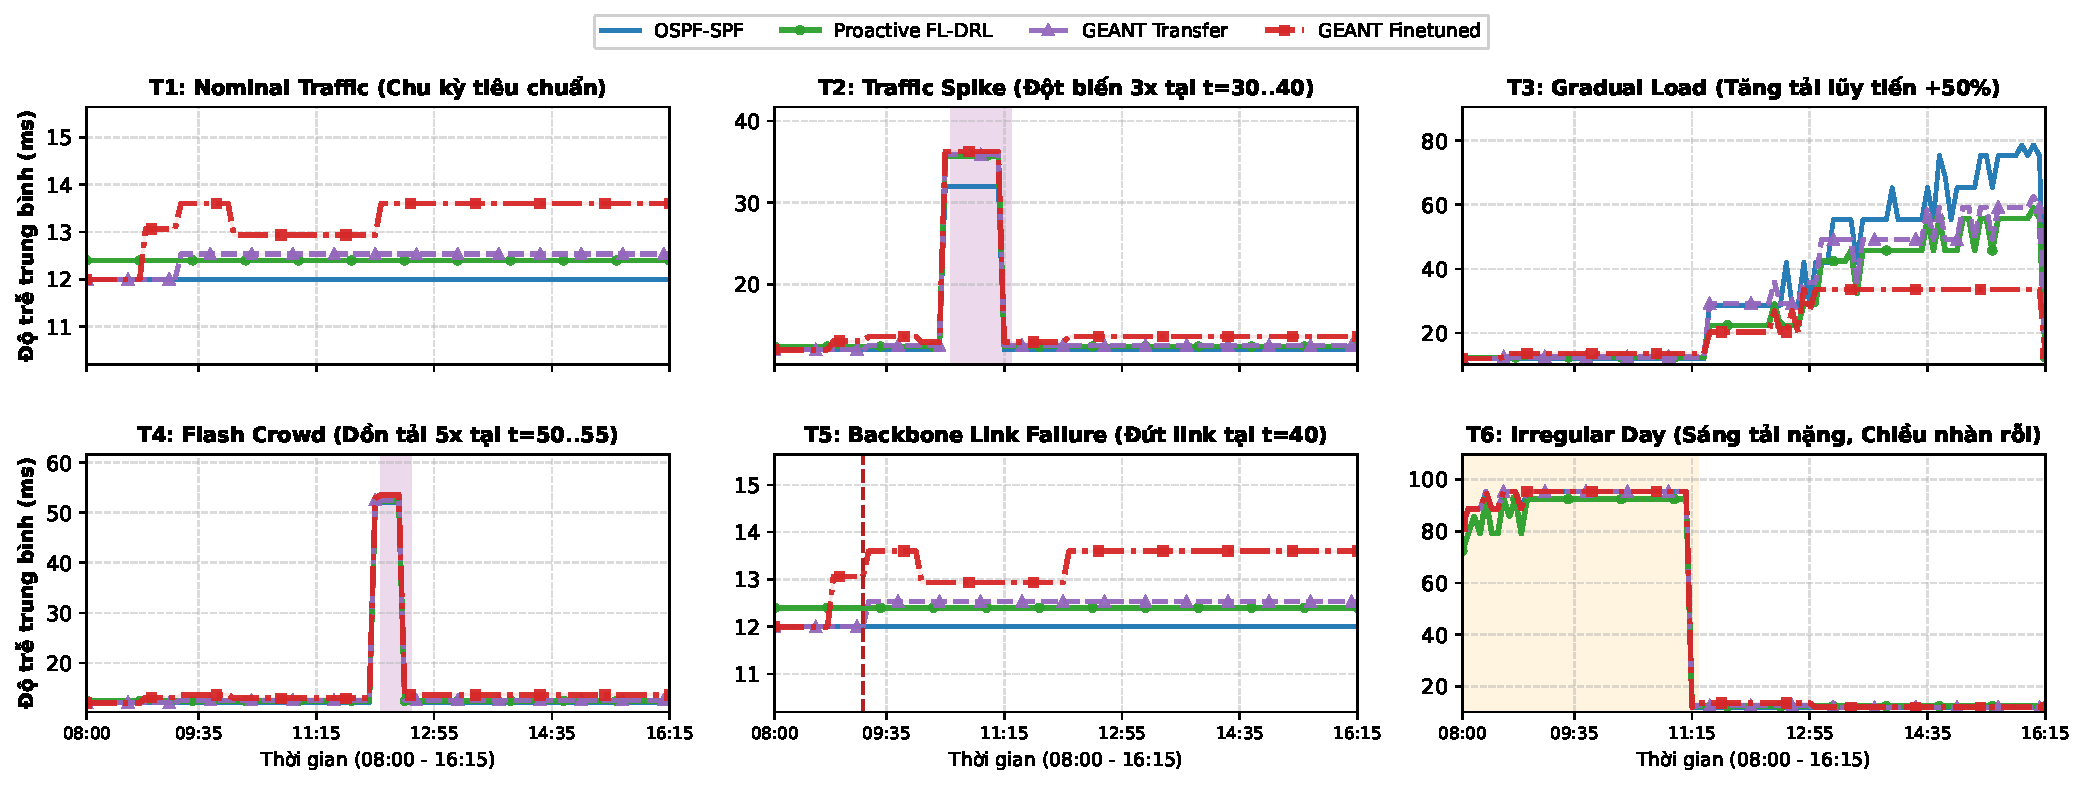
\includegraphics[width=\textwidth]{figures/overview_abilene_delay.pdf}
        \caption{Độ trễ trung bình (ms)}
    \end{subfigure}
    \vspace{0.15cm}
    \begin{subfigure}[b]{0.96\textwidth}
        \centering
        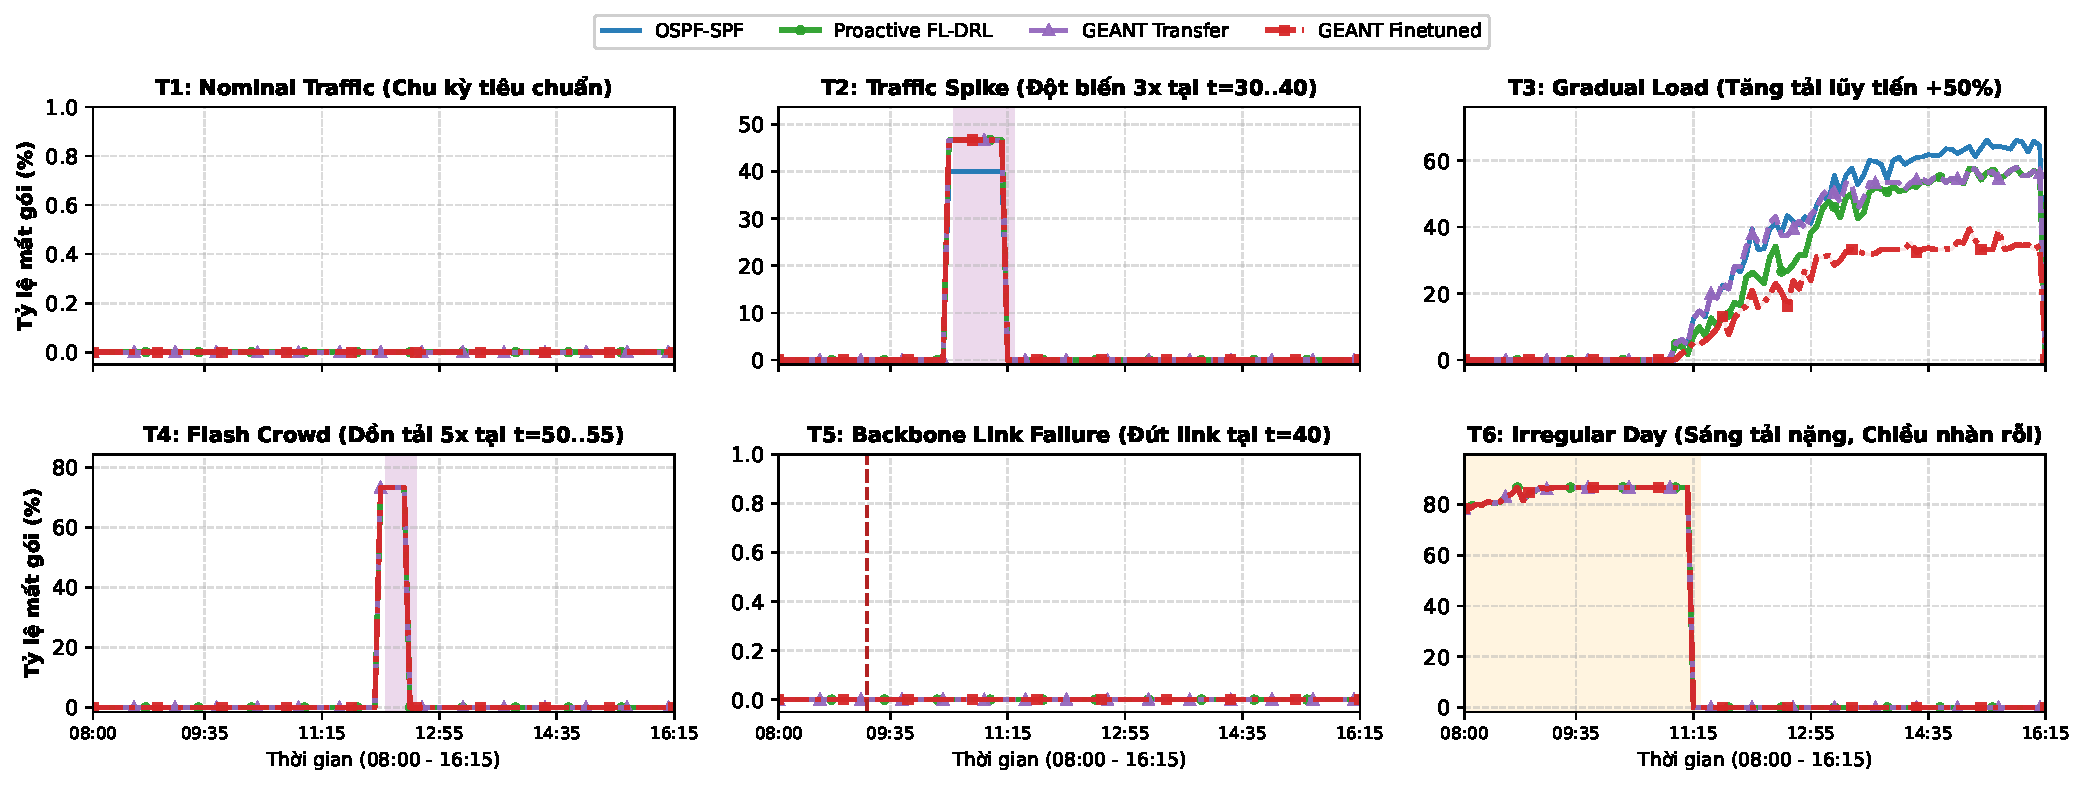
\includegraphics[width=\textwidth]{figures/overview_abilene_loss.pdf}
        \caption{Tỷ lệ mất gói (\%)}
    \end{subfigure}
    \caption{\textit{Toàn cảnh 6 kịch bản trên mạng Abilene: Đối sánh giữa OSPF, Mô hình Nội miền và GEANT Transfer (Lưới 2x3 vector chuẩn).}}
    \label{fig:abilene_all}
\end{figure}

\begin{itemize}[leftmargin=1.5em, itemsep=0.3ex]
    \item \textbf{Giải quyết trọn vẹn 14 điểm phản biện của GVHD:} Đã tiếp thu, giải trình khoa học và tích hợp hoàn chỉnh 14 nội dung kỹ thuật vào hệ thống nguyên mẫu (mô hình mạng và hàng đợi M/M/1, cấu trúc FL FedAdam, mô hình Gravity Model, vai trò khoa học của LSTM và RecurrentPPO, chiến lược Pareto 80/20, chuẩn hóa hàm Reward thích nghi, thuật toán step logic, đồ thị hội tụ 3 mạng, quy trình suy luận thời gian thực, cơ chế chuyển giao đa topo và phân tích trade-off độ trễ).
\end{itemize}

Hệ thống hiện có thể chạy hoàn chỉnh pipeline thử nghiệm và đánh giá tự động bằng script \texttt{run\_full\_pipeline.py} và \texttt{demo.py}, kết nối trực tiếp giữa môi trường mô phỏng, mô-đun FL và tác tử PPO, xuất đầy đủ dữ liệu CSV và đồ thị trực quan so sánh với OSPF.

% ==============================================================================
% 4. CÔNG VIỆC ĐANG THỰC HIỆN
% ==============================================================================
\section{Công việc đang thực hiện}

Hiện tại, nhóm đang tập trung thực hiện các nội dung công việc sau:
\begin{itemize}[leftmargin=1.5em, itemsep=0.3ex]
    \item \textbf{Hoàn thiện văn bản Báo cáo Khóa luận tốt nghiệp chi tiết:} Hệ thống hóa toàn bộ cơ sở lý thuyết, kiến trúc hệ thống, thuật toán FL/RL và phân tích chuyên sâu các bảng số liệu, biểu đồ thực nghiệm trên cả 3 mạng vào các chương theo quy định của Trường.
    \item \textbf{Mở rộng kiểm thử thực nghiệm trên Mininet thời gian thực:} Tiến hành đo đạc đối sánh với các luồng truyền video streaming UDP và lưu lượng TCP tải nặng để quan sát trực quan phản xạ tái định tuyến của Ryu Controller.
    \item \textbf{Chuẩn bị slide báo cáo và kịch bản demo:} Xây dựng bài thuyết trình bảo vệ khóa luận và hoàn thiện kịch bản demo trực quan trên giao diện giám sát mạng SDN.
\end{itemize}

% ==============================================================================
% 5. CÔNG VIỆC DỰ KIẾN TIẾP THEO
% ==============================================================================
\section{Công việc dự kiến tiếp theo}

Trong giai đoạn tiếp theo, các công việc dự kiến gồm:
\begin{itemize}[leftmargin=1.5em, itemsep=0.3ex]
    \item \textbf{Hoàn tất toàn bộ bản thảo khóa luận tốt nghiệp} và nộp phản biện theo đúng tiến độ của Khoa.
    \item \textbf{Báo cáo thử nghiệm và chạy demo kiểm tra} trước Giảng viên hướng dẫn để tiếp thu góp ý hoàn thiện.
    \item \textbf{Đóng gói mã nguồn}, cập nhật tài liệu hướng dẫn cài đặt và triển khai chi tiết trên GitHub phục vụ hội đồng chấm khóa luận.
\end{itemize}

\vspace{0.4cm}
Mã nguồn code: \url{https://github.com/Ragingsnake/ryu-fl-rl-traffic-controller}

\end{document}
